\documentclass[11pt]{article}

\usepackage{
    amssymb,
    amsmath,
    amsfonts,
    calc,
    eurosym,
    geometry,
    ulem,
    graphicx,
    caption,
    color,
    setspace,
    sectsty,
    comment,
    footmisc,
    caption,
    % natbib,
    pdflscape,
    subcaption,
    subfiles,
    titling,
    array,
    hyperref,
    booktabs,
    longtable,
    float,
    authblk,
    makecell,
    threeparttable}


\usepackage[
    backend=biber,
    style=nature,
    date=year,
    doi=true,
    isbn=false,
    url=false,
    eprint=false
]{biblatex}

\AtEveryBibitem{%
  \clearfield{note}%
}
\AtEveryCitekey{\clearlist{publisher}}
\AtEveryBibitem{\clearlist{publisher}}

\usepackage{pgf,tikz}
\usetikzlibrary{arrows, automata}
\usetikzlibrary{shapes.geometric,positioning}
\usetikzlibrary{positioning,calc}

\usepackage{siunitx}
\newcolumntype{d}{S[input-symbols = ()]}

\normalem

\renewcommand\Affilfont{\small\itshape}

\onehalfspacing
\newtheorem{theorem}{Theorem}
\newtheorem{corollary}[theorem]{Corollary}
\newtheorem{proposition}{Proposition}
\newtheorem{definition}{Definition}

\newenvironment{proof}[1][Proof]{\noindent\textbf{#1.} }{\ \rule{0.5em}{0.5em}}

\newtheorem{hyp}{Hypothesis}
\newtheorem{subhyp}{Hypothesis}[hyp]
\renewcommand{\thesubhyp}{\thehyp\alph{subhyp}}

\newcommand{\red}[1]{{\color{red} #1}}
\newcommand{\blue}[1]{{\color{blue} #1}}

\newcolumntype{L}[1]{>{\raggedright\arraybackslash}m{#1}}
\newcolumntype{C}[1]{>{\centering\arraybackslash}m{#1}}
\newcolumntype{R}[1]{>{\raggedleft\arraybackslash}m{#1}}
\subsubsectionfont{\normalfont\itshape}

\usepackage{mathtools}

\usepackage{letltxmacro}
\LetLtxMacro\orgvdots\vdots
\LetLtxMacro\orgddots\ddots

\makeatletter
\DeclareRobustCommand\vdots{%
  \mathpalette\@vdots{}%
}
\newcommand*{\@vdots}[2]{%
  % #1: math style
  % #2: unused
  \sbox0{$#1\cdotp\cdotp\cdotp\m@th$}%
  \sbox2{$#1.\m@th$}%
  \vbox{%
    \dimen@=\wd0 %
    \advance\dimen@ -3\ht2 %
    \kern.5\dimen@
    % remove side bearings
    \dimen@=\wd2 %
    \advance\dimen@ -\ht2 %
    \dimen2=\wd0 %
    \advance\dimen2 -\dimen@
    \vbox to \dimen2{%
      \offinterlineskip
      \copy2 \vfill\copy2 \vfill\copy2 %
    }%
  }%
}
\DeclareRobustCommand\ddots{%
  \mathinner{%
    \mathpalette\@ddots{}%
    \mkern\thinmuskip
  }%
}
\newcommand*{\@ddots}[2]{%
  % #1: math style
  % #2: unused
  \sbox0{$#1\cdotp\cdotp\cdotp\m@th$}%
  \sbox2{$#1.\m@th$}%
  \vbox{%
    \dimen@=\wd0 %
    \advance\dimen@ -3\ht2 %
    \kern.5\dimen@
    % remove side bearings
    \dimen@=\wd2 %
    \advance\dimen@ -\ht2 %
    \dimen2=\wd0 %
    \advance\dimen2 -\dimen@
    \vbox to \dimen2{%
      \offinterlineskip
      \hbox{$#1\mathpunct{.}\m@th$}%
      \vfill
      \hbox{$#1\mathpunct{\kern\wd2}\mathpunct{.}\m@th$}%
      \vfill
      \hbox{$#1\mathpunct{\kern\wd2}\mathpunct{\kern\wd2}\mathpunct{.}\m@th$}%
    }%
  }%
}
\makeatother


\newcommand{\ode}[2]{\frac{d{#1}}{d{#2}}}
\DeclareMathOperator{\E}{E}
\DeclareMathOperator{\indep}{\perp\!\!\!\perp}
\geometry{left=1.0in,right=1.0in,top=1.0in,bottom=1.0in}

\addbibresource{tnd.bib}

\begin{document}

\begin{titlepage}
\title{Identifying vaccine effectiveness in the test-negative design under an equi-confounding assumption\thanks{abc}}
\author[1]{ }
% \author[1]{Christopher Boyer\thanks{email: \href{mailto:cboyer@hsph.harvard.edu}{cboyer@hsph.harvard.edu}}}
% \affil[1]{Department of Epidemiology, Harvard T.H. Chan School of Public Health, Boston, MA.}
\date{\today}
\maketitle

\begin{abstract}
    The test-negative design (TND) is often used to monitor the effectiveness of vaccines under real-world conditions. In a TND study, individuals who develop the same symptoms and seek care are tested for the infectious disease of interest and effectiveness is estimated by comparing the vaccination history of test-positive and test-negative controls. Traditional approaches have justified the TND under the assumption that either a) receipt of a test is a perfect proxy for unmeasured (binary) health-seeking behavior or b) vaccination is unconfounded conditional on measured covariates, both of which are likely to be violated in practice. Here, we return to original motivation for the TND and show that the design may alternatively be justified under an assumption that unmeasured confounder(s) act equivalently for test positive and test negative controls on the odds ratio scale, i.e. odds ratio equi-confounding. We discuss the implications of this assumption for the design of TNDs. In addition to providing alternative justification for the conventional logistic regression estimator, we derive estimators for the marginal risk ratio among the vaccinated based on outcome modeling and inverse probability weighting using the generalized propensity score. We also derive a doubly-robust estimator allowing for the use of more flexible machine learning models. We provide proofs of our results as well as simulations to examine the finite sample performance of our estimators and illustrate the consequences when our assumptions are violated.
\noindent \\
\vspace{0in} \\
\noindent\textbf{Keywords:} test-negative design, vaccine effectiveness, causal inference, observational studies, unmeasured confounding, equi-confounding, odds ratios, selection bias
\bigskip
\end{abstract}
\setcounter{page}{0}
\thispagestyle{empty}
\end{titlepage}
\pagebreak \newpage

\doublespacing

\section{Introduction} \label{sec:introduction}
Observational data are frequently used for the post-market evaluation of vaccine effectiveness. Monitoring the effectiveness of vaccines is important as changes in population immunity as well as antigenic changes to the pathogen of interest occur that may render estimates from pre-market randomized trials irrelevant. Investigators may also be interested in the performance of vaccines in key populations that were ineligible or underrepresented in the clinical trial population; or they may want to compare vaccine formulations against one another or against other therapeutics not considered in the original trial. Under these circumstances, a quick and relatively cheap study design for estimating vaccine effectiveness is the so-called test-negative design (TND) \cite{sullivan_potential_2014,jackson_test-negative_2013}. 
 
Historically, the term ``test-negative design'' has been applied broadly to any design in which individuals who test positive for a pathogen of interest are compared with those who test negative. However, there are important methodological differences between approaches. Here, we focus on designs that meet the following criteria: patients with acute respiratory illness are prospectively recruited using a unified symptom screen through hospitals or other care facilities, consented, and a laboratory test for the pathogen of interest is preformed. Detailed information about their demographic, medical, and vaccination history is collected via a questionnaire at enrollment or through linked medical and vaccination records. Those who test positive form the ``cases'' and those who test negative are the comparison group. 

The TND was originally justified on the grounds that, in the presence of (unmeasured) binary healthcare-seeking behavior, the causal risk ratio against medically attended illness could be identified by the case status odds ratio among those screened and tested at a health facility, provided that the vaccine has no effect on the incidence of other respiratory illnesses that cause similar symptoms \cite{jackson_test-negative_2013}. It was also suggested that, by limiting to individuals who actually received a test, the TND may be less subject to measurement error \cite{jackson_test-negative_2013}. Subsequent work pointed out that the TND (i) is subject to residual confounding when healthcare-seeking is nonbinary \cite{sullivan_theoretical_2016,lewnard_theoretical_2021}, (ii) is subject to possible selection bias due to conditioning on the post exposure outcome of receiving a test \cite{sullivan_theoretical_2016}, and (iii) is biased when vaccination has a direct effect on testing behavior \cite{foppa_case_2013}. More recently, Schnitzer \cite{schnitzer_estimands_2022} suggested a formal causal framework for TND estimands and sampling design and showed that the marginal risk ratio is identified provided that observed covariates are sufficient to ensure no unmeasured confounding or selection bias. 

However, a question remains as to whether the TND is formally identified under weaker assumptions. In this article, we return to the original motivation for the TND and show that it may be alternatively justified under an assumption that unmeasured confounding is equivalent for test-positive cases and test-negative controls on the odds ratio scale. This assumption builds on the insight that infection with another respiratory illness, if plausibly unaffected by vaccination, is a negative outcome control in the population underlying the TND \cite{lipsitch_negative_2010,shi_selective_2020}. Therefore any observed differences in the incidence of other respiratory illnesses between vaccinated and unvaccinated individuals likely reflect residual confounding. If we assume equivalence between test-positive and test-negative infections, we can then use the negative outcome control to de-bias our estimate of vaccine effectiveness, similar to the parallel trends concept in the difference-in-differences literature \cite{sofer_negative_2016,park_universal_2023,tchetgen_universal_2023}. As we show, this insight extends to the biased sampling of the TND wherein only those who are tested are sampled, if we further assume that (potentially unobserved) determinants of test-seeking behavior are equivalent for test-positive and test-negative illnesses, which could be justified given the causative pathogen is presumably unknown to individuals prior to receiving a test. When our assumptions hold, we show that the traditional odds ratio estimator from the TND identifies the conditional risk ratio among the vaccinated in the population. We also derive new estimators of the marginal risk ratio among the vaccinated, including those based on outcome modeling and inverse probability weighting. We discuss the implications of our assumptions for the design of TNDs and provide proofs of our results as well as simulations to illustrate the consequences when our assumptions are violated.

\section{Setup and observed data} \label{sec:setup}
Let $X$ be a vector of baseline (pre-vaccination) covariates, $V$ an indicator of vaccination status, and $I$ a categorical indicator of symptomatic illness where
        $$I := \begin{cases} 
        I = 2 & \text{when infected by the pathogen of interest} \\
        I = 1 & \text{when infected by something else with same symptoms} \\
        I = 0 & \text{when no symptoms and/or uninfected}
        \end{cases}$$
Implicit in this assumption is that the infection events represented by $I = 1$ and $I = 2$ are mutually exclusive (this is relaxed in Appendix AX). Let $T$ be an indicator of receiving a test for the pathogen of interest (0/1), and $I^*$ the result of the test. For now, assume that we have access to a perfect test such that, for all individuals, $I^*_i = \mathbbm{1}(I_i = 2, T_i = 1)$, where $\mathbbm{1}(\cdot)$ is the indicator function. Extensions to cases where the test is imperfect are covered in Appendix AX but have been considered previously \cite{jackson2015effects}. Throughout we denote by $I^v$ the potential outcome under an intervention that sets vaccination to $V=v$. 
    
In a test-negative design, we assume the data are independent realizations of 
$$O = \{(X_i, V_i, S_i = 1, I^*_i) : i = 1, \ldots, n\}$$
where $S$ is an indicator of selection into test-negative design under potentially biased sampling from the underlying population. Selection is minimally based on presenting with a set of pre-specified symptoms at a health facility and receiving a test, i.e. $S = \mathbbm{1}(I \neq 0, T = 1)$, but could be extended to include other criteria such as hospitalization or severe disease. We assume that the screen is effective such that everyone tested has either $I=1$ or $I=2$. Vaccination status and associated covariates may be retrospectively assessed at the time of testing or, preferably, pulled from outside sources such as vaccine registries or healthcare databases. 

\section{Causal estimands for the test-negative design} \label{sec:estimands}
In the TND literature, the target parameter is generally the causal risk ratio,
\begin{equation*}
    \Psi_{RR} \equiv \dfrac{\Pr[I^1 = 2]}{\Pr[I^0 = 2]},
\end{equation*}
which contrasts the probability of symptomatic infection if everyone in the population underlying the TND were vaccinated compared to if they were unvaccinated, with ``vaccine effectiveness'' against symptomatic infection defined as $1 - \Psi_{RR}$. When there is no direct effect of vaccination on testing (formalized below), then $\Psi_{RR}$ is equivalent to the causal risk ratio for \textit{testing positive} with symptomatic illness,
\begin{equation*}
    \Psi_{RR} = \dfrac{\Pr[I^1 = 2, T^1 = 1]}{\Pr[I^0 = 2, T^0 = 1]}.
\end{equation*}
Note, this could be the estimand, for instance, in a randomized trial in which participants present naturally for testing when they develop symptoms rather than being randomly sampled and tested regardless of symptoms on a given follow up day. In previous work, this is sometimes referred to as medically-attended illness \cite{jackson_test-negative_2013}, under the presumption that to receive a test requires sufficiently acute disease to warrant seeking care. As shown by \Citeauthor*{schnitzer_estimands_2022} \cite{schnitzer_estimands_2022}, under the assumptions that measured covariates $X$ are sufficient to control confounding and selection bias, the odds ratio comparing vaccination among test-positive cases and test-negative controls under the biased sampling of the test-negative design is a consistent estimator of $\Psi_{RR}$. In practice, effectiveness is often estimated via a logistic regression which conditions on $X$ in which case the estimand is more appropriately the conditional risk ratio,
\begin{equation*}
    \Psi_{RR}(X) \equiv \dfrac{\Pr[I^1 = 2 | X]}{\Pr[I^0 = 2 | X]}.
\end{equation*}

Here, we relax the typical no-unmeasured confounding assumption, but to do so requires that we focus instead on the causal risk ratio \textit{among the vaccinated}, i.e.
\begin{equation*}
    \Psi_{RRV} \equiv \dfrac{\Pr[I^1 = 2 | V = 1]}{\Pr[I^0 = 2 | V = 1]} .
\end{equation*}
rather than the risk ratio in the full population. This is similar to the average treatment effect on the treated in the causal inference literature. When vaccination provides constant protection for everyone, $\Psi_{RRV}$ this will be equivalent to the causal risk ratio in the full population, i.e. $\Psi_{RR} = \Psi_{RRV}$. However, when vaccination provides heterogeneous protection, the causal risk ratio in the full population will be a weighted average of the causal risk ratio among the vaccinated and unvaccinated.

\section{Identification} \label{sec:identification}
\subsection{Identifiability conditions} \label{sec:conditions}
We consider the identification of the causal risk ratio among the vaccinated, $\Psi_{RRV}$, under the following conditions
\begin{itemize}
    \item[(A1)] Consistency of potential outcomes. For all individuals $i$ and for $v \in \{0, 1\}$, we have $I_i^v = I_i$ and $T_i^v = T_i$ when $V_i = v$.
    \item[(A2)] No effect of vaccination on symptomatic illness for non-target pathogen ($I = 1$) among the vaccinated. That is, $\Pr[I^0 = 1 | V = 1, X] = \Pr[I^1 = 1 | V = 1, X].$
    \item[(A3)] Odds ratio equi-confounding. Degree of unmeasured confounding bias on the odds ratio scale is the same for all symptomatic illness regardless if $I=1$ or $I=2$ is cause, i.e. 
    $$OR_2(X) = OR_1(X), $$
    $$ \text{where } OR_i(X) = \frac{\Pr[I^0 = i, T^0 = 1 | V = 1, X]\Pr[I^0 = 0, T^0 = 1 | V = 0, X]}{\Pr[I^0 = 0, T^0 = 1 | V = 1, X]\Pr[I^0 = i, T^0 = 1| V = 0, X]}.$$
    \item[(A4)] Overlap of vaccination among test-positives and test-negatives. Define $\mathcal{S}_i(v)$ as the support of the law of $(I^v = i, T^v = 1, V = v, X)$, then for $v$ in $\{0,1\}$, then it must be that $\mathcal{S}_2(1) \subseteq \mathcal{S}_2(0)$ and $\mathcal{S}_2(v) \subseteq \mathcal{S}_1(v).$
    \item[(A5)] No direct effect of vaccination on test-seeking behavior among the vaccinated. That is, for $i$ in $\{1,2\}$, $\Pr[T^1 = 1 | I^1 = i, V = 1, X] = \Pr[T^0 = 1 | I^0 = i, V = 1, X].$
\end{itemize}

Assumptions (A1) and (A4) are well-known identifiability conditions discussed in more detail elsewhere \cite{hernan_causal_2020}. Assumption (A2) implies that the vaccine does not provide any cross-protection against other types of infection which may cause the same symptoms. It may be violated if vaccination provides short-term nonspecific protection through activation of the immune system. In principle, this assumption could be evaluated in a randomized vaccine trial by measuring incidence of other respiratory illnesses, although in practice trials may not be adequately powered to rule out small effects. Assumption (A5) requires that an individual's decision to seek care and get tested is not affected by their vaccination status (although it can depend on other measured and unmeasured characteristics). In a placebo-controlled trial, it is ensured through the blinding of the participant to their vaccination status. Both (A2) and (A5) have been invoked in the previous literature formalizing the test-negative design \cite{jackson_test-negative_2013,schnitzer_estimands_2022}. In Appendix AX, we show that assumption (A5) can be further relaxed provided the effect of vaccination on testing is equivalent for test-positive and test-negative illnesses.

Assumption (A3) is the key assumption of this paper and is an alternative to the conditional independence conditions suggested previously \cite{schnitzer_estimands_2022}. It states that the degree of unmeasured confounding on the odds ratio scale is the same for illnesses with the same symptom set regardless if $I=2$ or $I=1$ is the cause. Notably, it does not impose other restrictions such that the unmeasured confounder(s) must be binary or even related to health-seeking specifically (although health-seeking behavior is a credible candidate for satisfying A3). \citeauthor{lewnard_measurement_2018} briefly discussed identification under a similar condition, although not in a formal causal framework \cite{lewnard_measurement_2018}. It is also similar, in spirit, to a recently suggested  scale-independent alternative to the parallel trend assumption in the difference-in-differences literature \cite{park_universal_2023,tchetgen_universal_2023}. Note that, when $I = 1$ and $I = 2$ are mutually exclusive, we can simplify (A3) to
\begin{equation}
    \frac{\Pr[I^0 = 2, T^0 = 1 | V = 1, X]}{\Pr[I^0 = 2, T^0 = 1 | V = 0, X]} =\frac{\Pr[I^0 = 1, T^0 = 1 | V = 1, X]}{\Pr[I^0 = 1, T^0 = 1 | V = 0, X]}
\end{equation}
Furthermore, by a simple factorization we can split (A3) into alternative assumptions (A3a) and (A3b), emphasizing the dual influences of confounding of the effect of vaccination on symptomatic illness and selection related to receiving a test:
\begin{itemize}
    \item[(A3a)] Odds ratio equi-confounding. Degree of unmeasured confounding bias on the odds ratio scale is the same for symptomatic illness regardless if $I=1$ or $I=2$ is cause, i.e. 
    $$\frac{\Pr[I^0 = 2 | V = 1, X]}{\Pr[I^0 = 2 | V = 0, X]} =\frac{\Pr[I^0 = 1 | V = 1, X]}{\Pr[I^0 = 1 | V = 0, X]}.$$
    \item[(A3b)] Odds ratio equi-selection. Degree of unmeasured selection bias, e.g. receiving a test, on the odds ratio scale is the same for all symptomatic illness regardless if $I=1$ or $I=2$ is cause, i.e. 
    $$\frac{\Pr[T^0 = 1 | I^0 = 2, V = 1, X]}{\Pr[T^0 = 1 | I^0 = 2, V = 0, X]} =\frac{\Pr[T^0 = 1 | I^0 = 1, V = 1, X]}{\Pr[T^0 = 1 | I^0 = 1, V = 0, X]}.$$
\end{itemize}
In section X of the Appendix, we provide example data generation mechanisms that satisfy the odds ratio equi-confounding assumptions as well as those in which the assumptions are violated to provide further intuition.

\subsection{Graphical criteria} \label{sec:graphical}
The causal directed acyclic graphs (DAGs) in Figure 1 represent possible data generating mechanisms underlying the test-negative design. Here we add $U$ to the previous setup representing a possible unmeasured confounder. The DAGs in Figure 1a and 1b show mechanisms discussed previously in the TND literature. Figure 1a is a modified version of the DAG in \citeauthor{schnitzer_estimands_2022} \cite{schnitzer_estimands_2022}, where the assumption of no unmeasured confounding or selection bias is shown by the lack of an arrow from $U$ to $V$. Assumption (A5) is also shown by the lack of a direct arrow from $V$ to $T$, implying no direct effect of vaccination on testing behavior. Figure 1b is a modified version of the DAG in \citeauthor{sullivan_theoretical_2016} \cite{sullivan_theoretical_2016}, where $U$ is binary health seeking behavior that is synonymous with receiving a test and therefore effectively conditioned on by conditioning on testing.  

The DAG in Figure 1c shows a possible mechanism satisfying the identifiability conditions in this study. It includes the possibility of unmeasured confounding and selection bias, as there is now an arrow from $U$ to $V$; however, as shown by the bold arrows $U$ is assumed to act equivalently, on the odds scale, for the test positive and test negative illnesses. This condition imposes a parametric restriction on the allowable data generation mechanisms implied by the DAG and as such requires nonstandard notation. The DAGs in Figures 1c and 1d depict alternative mechanisms in which only equi-confounding, Assumption (A3a), or equi-selection, Assumption (A3b), are assumed. In Figure 2, we show an alternative DAG that splits the $I$ node into $I_1 = \mathbbm{1}(I = 1)$ and $I_2 = \mathbbm{1}(I = 2)$ with the dashed arrow between them representing the deterministic relationship as they are assumed to be mutually exclusive. This graph allows us to show assumption (A2) by the lack of a directed arrow between $V$ and $I_1$. 

\subsection{The test-negative illness as a proxy for unmeasured confounding} \label{sec:effect_among_vaccinated}
To build intuition about identification under these conditions, we ignore the sampling design of the TND for now and consider the conditional risk ratio for testing-positive among the vaccinated in the underlying cohort, i.e.
\begin{equation*}
    \Psi_{RRV}(X) \equiv  \frac{\Pr[I^1 = 2 | V = 1, X]}{\Pr[I^0 = 2 | V = 1, X]} &= \frac{\Pr[I^1 = 2, T^1 = 1 | V = 1, X]}{\Pr[I^0 = 2, T^0 = 1 | V = 1, X]}.
\end{equation*}
Multiplying by the constant $\frac{\Pr[I = 2, T = 1| V = 0, X]}{\Pr[I = 2, T = 1 | V = 0, X]}$ and applying consistency assumption (A1) for the numerator, we find that $\Psi_{RRV}(X)$ satisfies:
\begin{align*}
    \Psi_{RRV}(X) &=\underbrace{\frac{\Pr[I = 2, T = 1 | V = 1, X]}{\Pr[I = 2, T = 1 | V = 0, X]}}_{\text{observed risk ratio}} \times \underbrace{\frac{\Pr[I = 2, T = 1 | V = 0, X]}{\Pr[I^0 = 2, T^0 = 1 | V = 1, X]}}_{\text{de-biasing term}} 
\end{align*}
where this expression decomposes the causal risk ratio among the vaccinated into the (crude) observed risk ratio and a de-biasing term quantifying the difference in vaccination-free outcome of testing positive with symptomatic infection between those who were vaccinated and those who were not. If there is no unmeasured confounding for symptomatic infection or receving a test, then the de-biasing term is equal to one and the observed risk ratio is equal to the causal risk ratio among the vaccinated. If there is unmeasured confounding, then the de-biasing term is the quantity that would be necessary to remove the bias from the observed risk ratio but it depends crucially on the unobserved quantity $\Pr[I^0 = 2, T^0 = 1 | V = 1, X]$, i.e. the counterfactual probability of symptomatic infection and receiving a test among the vaccinated if, contrary to the fact, they had not been vaccinated. 

The logic behind the equi-confounding assumption, therefore, is to use the test-negative controls as a proxy for the unobservable quantity $\Pr[I^0 = 2, T^0 = 1 | V = 1, X]$. This could be justified on the grounds that the test negative controls exhibit a similar joint propensity for illness and health-seeking, but should not be affected by the vaccine (as the vaccine is assumed to have no effect on symptomatic illness arising from other pathogens). Thus any residual difference in the incidence of the test-negative illness between vaccinated and unvaccinated individuals after conditioning on covariates must reflect unmeasured confounding. Under equi-confounding it is assumed that these unmeasured factors act equivalently on infection and testing for $I=1$ and $I=2$ on the odds ratio scale and therefore the ratio of $I=1$ among vaccinated and unvaccinated may be used to recalibrate the observed risk ratio for $I = 2$. More specifically, as we show in the Appendix, by combining the equi-confounding assumption with the other assumptions in section, we have
    \begin{equation}\label{eqn:proxy}
     \Pr[I^0 = 2, T^0 = 1  | V = 1, X] = \frac{\Pr[I = 1, T = 1  | V = 1, X]}{\Pr[I = 1, T = 1  | V = 0, X]}\Pr[I = 2, T = 1 | V = 0, X],
    \end{equation}
where we note that $\frac{\Pr[I = 1, T =1  | V = 0, X]}{\Pr[I = 1, T = 1 | V = 1, X]}$ acts as a proxy for $\frac{\Pr[I^0 = 2, T^0 =1  | V = 0, X]}{\Pr[I^0 = 2, T^0 = 1 | V = 1, X]}$ or, borrowing from the difference-in-differences literature, essentially a ``parallel trend'' for $I=2$ in absence of vaccination. This is similar to the intuitive motivation for the test-negative design, i.e. that those who test-negative are, for a variety of reasons related to care-seeking etc, a useful proxy for the test-positives. 

Plugging the result in equation \ref{eqn:proxy} back into the definition of $\Psi_{RRV}(X)$, we obtain the following 
    \begin{equation}
         \Psi^\dagger_{om}(X) \equiv \dfrac{\dfrac{\Pr[I = 2, T = 1 | V = 1, X]}{\Pr[I = 1, T = 1 | V = 1, X]}}{\dfrac{\Pr[I = 2, T = 1 | V = 0, X]}{\Pr[I = 1, T = 1 | V = 0, X]}}
    \end{equation}
which is the odds ratio comparing the odds of testing positive with the test-positive or test-negative illness in the vaccinated and unvaccinated. Note, $\Psi^\dagger_{om}(X)$ is written strictly in terms of observable quantitites.

\subsection{Efficient sampling of outcome and proxy via the test-negative design}
If we had access to the complete testing data in the cohort underlying the TND, $\Psi^\dagger_{om}(X)$ would be identified without further effort. However, recall that in a TND we observe, potentially biased, samples from the tested only, i.e. we observe samples from $(X_i, V_i, S_i = 1, I^*_i)$ for $i = 1, \ldots, n$ where $S_i = \mathbbm{1}(I_i \neq 0, T_i = 1)$. Nonetheless, as we show in Appendix X, $\Psi^\dagger_{om}(X)$ is equivalent to 
    \begin{equation}\label{eqn:or_estimand}
         \Psi^*_{om}(X) = \dfrac{\dfrac{\Pr[I^* = 1 | S = 1, V = 1, X]}{\Pr[I^* = 0 | S = 1, V = 1, X]}}{\dfrac{\Pr[I^* = 1 | S = 1, V = 0, X]}{\Pr[I^* = 0 | S = 1, V = 0, X]}}
    \end{equation}    
which is the odds ratio comparing odds of testing positive for vaccinated and unvaccinated \textit{among the tested} and is identified under the biased sampling design of the TND. This result follows, essentially, from the invariance of the odds ratio $\Psi^\dagger_{om}(X)$. As discussed below, $\Psi^*_{om}(X)$ is a possible target of the commonly used logistic regression estimator in TND studies, provided it is correctly specified. This suggests that estimates based on logistic regression from existing studies could be alternatively justified under an equi-confounding assumption. Note that, under our setup the the TND can be viewed as, essentially, an efficient sampling of the outcome and negative outcome control from the underlying cohort.

\subsection{Full identification results for the risk ratio among the vaccinated}
In practice, the effectiveness of the vaccine may vary across important subgroups in the population. For instance, effectiveness against symptomatic infection may be lower for those in older age groups or among those with weakened immune systems or other comorbidities. Although the risk ratio is collapsible, in principle, in the full population, the biased sample of the TND requires special attention. As we show in Appendix A1, under assumptions A1 - A5 and the biased sampling design of the test-negative study, the marginal risk ratio among the vaccinated, $\Psi_{RRV}$, is identified by
\begin{equation}\label{eqn:om_estimand}
    \Psi_{om}^* = \dfrac{\Pr(I^* = 1 | S = 1, V = 1)}{E\left\{  \dfrac{\Pr(I^* = 0 | S = 1, V = 1, X)}{\Pr(I^* = 0| S = 1, V = 0, X)}\Pr(I^* = 1 | S = 1, V = 0, X) \Big| S = 1, V = 1 \right\}}
\end{equation}
or alternatively 
\begin{equation}\label{eqn:ipw_estimand}
    \Psi_{ipw}^* = \dfrac{E\{VI^*|S =1\}}{E\left\{ (1 - V) I^* \dfrac{\pi^*(X)}{1 - \pi^*(X)} \bigg| S = 1\right\}}
\end{equation}
where $\alpha^*_1(X) = \dfrac{\Pr(I^* = 0 | S = 1, V = 1, X)}{\Pr(I^* = 0| S = 1, V = 0, X)}$ and $\pi^*(X) = \Pr(V = 1| S = 1, I^* = 0, X)$. Expression (\ref{eqn:om_estimand}) generalizes the result in expression (\ref{eqn:or_estimand}), where now the denominator is standardized over the distribution of $X$ among the vaccinated in the TND sample. Expression \ref{eqn:ipw_estimand} is motivated again by the invariance property of the odds ratio where, by Assumption (A3), 
$$\frac{\Pr[V = 1 | I^0 = 2, T^0 = 1, X]}{\Pr[ V = 0 | I^0 = 2, T^0 = 1, X]} =\frac{\Pr[V = 1 | I^0 = 1, T^0 = 1, X]}{\Pr[V = 0 | I^0 = 1, T^0 = 1, X]}$$
which implies the odds of vaccination in the test-negative controls are a proxy for the so-called \textit{extended propensity score} (EPS) function, $\pi^*(X)$. The EPS extends the standard propensity score function to accommodate unmeasured confounding by conditioning on the treatment-free potential outcomes $I^0 = 2$ and $T^0 = 1$. 

\section{Estimation}
The traditional approach to estimating vaccine effectiveness in a TND is based on logistic regression for $I^*$ conditional on $X$ and $V$, e.g.
$$\log \left\{\dfrac{\Pr[I^* = 1 | S = 1, V, X]}{\Pr[I^* = 0 | S = 1, V, X]}\right\} = \gamma_0 + \gamma_1 V + \gamma_2 X,$$
where effectiveness is defined as one minus the odds ratio comparing vaccinated and unvaccinated, i.e. $VE = 1 - \exp(\gamma_1)$. As we have shown, $ \exp(\gamma_1)$ is equal to $\Psi^*_{om}(X)$ and by extension the conditional causal risk ratio among the vaccinated $\Psi_{RRV}(X)$ under the identifiability assumptions of Section \ref{sec:conditions} and correct model specification. 

Alternatively, expressions (\ref{eqn:om_estimand}) and (\ref{eqn:ipw_estimand}) suggest two plug-in estimators which are valid under effect modification. Expression (\ref{eqn:om_estimand}) suggests an estimator based on modeling the outcome
\begin{equation}\label{eqn:om_estimator}
    \widehat{\Psi}_{om}^* = \dfrac{\sum_{i=1}^n V_i I^*_i}{\sum_{i=1}^n V_i \widehat{\mu}_0(X_i)\dfrac{1 - \widehat{\mu}^*_1(X_i)}{1 - \widehat{\mu}^*_0(X_i)}},
\end{equation}
where $\mu^*_v(X) &= \Pr(I^*=1\mid S=1, V=v, X)$ is the probability of testing positive among those with vaccine status $V =v$ in the TND sample, and expression (\ref{eqn:ipw_estimand}) suggests an inverse probability weighting estimator
\begin{equation}\label{eqn:ipw_estimator}
    \widehat{\Psi}_{ipw}^* = \dfrac{\sum_{i=1}^n V_i I^*_i}{\sum_{i=1}^n (1 - V_i) I^*_i \dfrac{\pi^*(X_i)}{1 - \pi^*(X_i)}},
\end{equation}
where $\pi^*(X) = \Pr(V=1\mid S=1, I^*=0, X)$ is the probability of vaccination among the test-negative controls. The first estimator, $\widehat{\Psi}_{om}^*$, requires the correct specification of the model for the outcome and the second estimator, $\widehat{\Psi}_{ipw}^*$,  requires the correct specification of the the model for the extended propensity score model. In some settings, one estimator may be preferred over the other. For instance, when more is known about the mechanism for ``assigning'' vaccination, the weighting estimator may be preferred \cite{robins_estimating_1992,braitman_rare_2002}; when the process that gives rise to infection and testing is well understood the outcome estimator may be preferred. In practice, however, both models may be difficult to specify correctly. Using data-adaptive and more flexible machine learning estimators for estimation of these nuisance models offers the possibility of capturing more complex data generation processes. These data-adaptive estimators generally have slower rates of convergence than the $\sqrt{n}$ rates of parametric models and therefore will not yield asymptotically valid confidence intervals \cite{chernozhukov_doubledebiased_2018}. To address this challenge, we can use a doubly-robust estimator which combines models for the conditional loss $\widehat{\mu}^*_v(X)$ and the probability of treatment $\widehat{\pi}^*(X)$. In Appendix AX, we derive such an estimator based on the efficient influence function for $\Psi_{RRV}$
\begin{equation}\label{eqn:dr_estimator}
    \widehat{\Psi}_{dr}^* = \dfrac{\sum_{i=1}^n V_i I^*_i}{\sum_{i=1}^n (1 - V_i)\dfrac{\pi^*_1(X_i)}{1 - \pi^*_1(X)} \{I_i - \mu^*_0(X_i) \} + V_i \mu^*_0(X_i)\dfrac{1 - \mu^*_1(X_i)}{1 - \mu^*_0(X_i)}}
\end{equation}

\section{Sensitivity analysis}
In practice, the odds ratio equi-confounding assumption may not hold such that
$$OR_2(X) \neq OR_1(X).$$ 
However, the decomposition in expression Z suggests a sensitivity analysis which allows for a straightforward departure from equi-confounding as follows. Consider the case that the odds ratio function $OR_2(X)$ is, instead, equal to
$$ OR_2(X) = e^{\eta q(X)} OR_1(X) $$
where $\eta$ is a scalar and $q(X)$ is user-specified a monotone sensitivity function which, when combined, parameterize the departure from equi-confounding on the odds ratio scale. This is an example of the well-known exponential tilt model. Setting $\eta = 0$ corresponds to the case where equi-confounding holds and values of $\eta$ further from zero represent larger violations. For instance, one might specify $q(X) = 1$, which suggests that confounding occurs equally across levels of $X$, and then vary $\eta$ over a grid of values in the interval $(-\omega, \omega)$. For each value of $\eta$, the analysis is repeated and updated estimates of $\Psi$ are obtained. The resulting set of estimates can be used to construct a confidence interval for $\Psi$ that is robust to violations of the equi-confounding assumption.

\section{Simulation}

To illustrate a data generation process where our assumptions hold and to verify the empirical performance of the proposed estimators when they do not, we perform a simulation study mimicking a TND with binary vaccination, testing, and, infection. We consider the following data generation process:
\begin{align*}
    X, U &\sim \text{Unif}(0,1)\\
    V\mid X, U & \sim \text{Bernoulli}(\expit(\alpha_0 + \alpha_X X + \alpha_U U))\\
    I \mid V, X, U &\sim \text{Multinomial}(1-p_1(V, X, U), p_1(V, X, U), p_2(V, X, U))\\
    T\mid I, V, X, U &\sim \text{Bernoulli}(\mathbbm 1(I>0)\exp\{\tau_{1}\mathbbm 1(I=1) + \tau_{2}\mathbbm 1(I=2) + \tau_V V + \tau_X X \\&\qquad \qquad\qquad + \tau_U U + \tau_{2U} U \mathbbm 1(I=2) + \tau_{2V} V \mathbbm 1(I=2) \})
\end{align*}
where $U$ is an unmeasured confounder and
\begin{align*}
    p_1(V, X, U) & = \Pr[I = 1 | V, X, U] = \exp(\beta_{10} + \beta_{1V}V + \beta_{1X}X + \beta_{1U}U) \\
    p_2(V, X, U) & = \Pr[I = 2 | V, X, U] = \exp(\beta_{20} + \beta_{2V}V + \beta_{2X}X + \beta_{2U}U).
\end{align*}
This setup means the potential outcomes $(I^v, T^v)$ for $v=0,1$ and $i=1, 2$ are generated from
\begin{align*}
    \Pr[I^v=0, T^v=1\mid V, X, U] &= 0\\
    \Pr[I^v=i, T^v=1\mid V, X, U] &= p_i(v, X, U)\exp\{\tau_i + \tau_V v + \tau_X X + \tau_U U \\&\qquad \qquad\qquad + \tau_{2U}U\mathbbm 1(I^v=2) + \tau_{2V} v \mathbbm 1(I^v=2) \}.
\end{align*}
which implies the conditional independence $I^v, T^v\indep V\mid X, U$ holds for $v=0,1$, i.e. conditioning on $U$ and $X$ would be sufficient to control confounding. Furthermore, 
\begin{align*}
    \dfrac{\Pr[I^0=2, T^0=1 \mid V=1,X]}{\Pr[I^0=2, T^0=1\mid V=0,X]}=\dfrac{\E[\exp\{(\tau_U  + \tau_{2U}+\beta_{2U})U\}\mid V=1, X]}{\E[\exp\{(\tau_U  + \tau_{2U}+\beta_{2U})U\}\mid V=0, X]}
\end{align*}
and 
\begin{align*}
    \dfrac{\Pr[I^0=1, T^0=1 \mid V=1,X]}{\Pr[I^0=1, T^0=1\mid V=0,X]}=\dfrac{\E[\exp\{(\tau_U  +\beta_{1U})U\}\mid V=1, X]}{\E[\exp\{(\tau_U +\beta_{1U})U\}\mid V=0, X]}
\end{align*}
implying that Assumtion (A4) holds when $\beta_{2U}=\beta_{1U}$ and $\tau_{2U}=0$. We note that in our setting, Assumption (A4) can be viewed as composed of two conditions: the unmeasured confounding bias for two illness outcomes have equal size ($\beta_{1U}=\beta_{2U}$), and there is no interaction between unmeasured confounder and illness outcome in the risk of testing on a multiplicative scale ($\tau_{2U}=0$). Furthermore, $\beta_{1V}=0$ controls whether there is a direct effect of vaccination on $I = 1$, i.e. Assumption (A2). Without this assumption, we may at best identify the difference of vaccine effects on the two illness outcomes, i.e. $\beta_{2V}-\beta_{1V}$. The parameter $\tau_V$ controls whether there is a direct effect of vaccination on $T$, i.e. Assumption (A3).%\textcolor{red}{TODO: Is (A3) necessary?}

We generate a target population of $N = 10,000$ resulting in TND samples of test-positive cases and test-negative controls of between $2000$ and $3000$. We consider nine scenarios: (1) no unmeasured confounding; (2) unmeasured confounding but assumptions (A1)-(A5) hold; (2) equi-confounding holds but equi-selection does not; (3) equi-selection holds but equi-confounding does not; (4) neither equi-confounding nor equi-selection hold; (5) equi-confounding and equi-selection hold but there is a direct effect of vaccination on $I = 1$; (6) equi-confounding and equi-selection hold but there is an equal effect of vaccination on $T$; (7) equi-confounding and equi-selection hold but there is an unequal effect of vaccination on $T$; and (9) all assumptions hold but there is effect modification by covariates $X$. For each scenario, we generate 1000 replicates and estimate the causal risk ratio among the vaccinated using the proposed estimator and calculate the bias and coverage of 95\% confidence intervals based on the true value. For comparison, we also estimate the causal risk ratio among the vaccinated assuming one had access to the full sample in the target population, as in a cohort study. We consider both the more typical case that the covariate $U$ is unmeasured and unavailable and the hypothetical case that $U$ is available and therefore the a sufficient adjustment set can therefore be conditioned on. 

The results are reported in Figure \ref{fig:sims}. When there is no unmeasured confounding, all estimators are unbiased. In all other scenarios the typical cohort estimator without $U$ is biased. When there is unmeasured confounding but assumptions (A1)-(A5) hold, the TND estimator is unbiased. When there is an effect of vaccination on the test-negative illness, the TND estimator is biased; however, it does identify the ratio of vaccine effects against $I = 2$ versus $I = 1$. When equi-confounding or equi-selection are violated the TND estimator is biased. When the the test-negative and test-positive illnesses are not mutually exclusive, the TND estimator is biased for the causal risk ratio but unbiased for the causal odds ratio.  When there is a direct effect of vaccination on testing behavior, the TND estimator remains unbiased if the effect is equivalent for test-negative and test-positive illnesses, but is biased when they are unequal. Finally, the TND estimator remains unbiased in the presence of effect modification. %When there is unmeasured confounding and equi-confounding holds but equi-selection does not, the proposed estimator is biased but has good coverage. When there is unmeasured confounding and equi-selection holds but equi-confounding does not, the proposed estimator is unbiased but has poor coverage. When there is unmeasured confounding and neither equi-confounding nor equi-selection hold, the proposed estimator is biased and has poor coverage. When there is unmeasured confounding and equi-confounding and equi-selection hold but there is a direct effect of vaccination on $I = 1$, the proposed estimator is biased and has poor coverage. When there is unmeasured confounding and equi-confounding and equi-selection hold but there is a direct effect of vaccination on $T$, the proposed estimator is biased and has poor coverage.

\section{Discussion} \label{sec:discussion}

In this article, we have described alternative identifiability conditions under which the test-negative design produces an unbiased estimate of the vaccine effectiveness against symptomatic illness. Our results allow for the possibility of unmeasured confounding provided that the degree of confounding is the same for the illnesses 

Requires knowledge of what the test-negative illness or illnesses are in order to understand whether equi-confounding is plausible. In some sense the ideal comparator would be an illness with a similar transmission mechanism/exposure mechanism and a similar presentation, but is unaffected by the vaccine. Some examples of unmeasured characteristics where equi-confounding may hold include health-seeking, assortativity. In previous work on flu the most common test-negative illnesses were X.  

We have mainly focused on TND in the outpatient setting, where voluntary care seeking is
Our approach is 
Our results rely crucia

Our results also rely on the assumption that the vaccine does not affect the incidence of other infections which may cause the same symptoms. This assumption may be violated if either vaccination or infection provides short-term nonspecific protection through activation of the immune system. Previous work has suggested that this may be the case for influenza vaccines \cite{cowling_increased_2012}. However, other results have shown the opposite \cite{sundaram_influenza_2013}.

Prior work on the TND suggests that the design could be biased when there is correlation in vaccination behavior for vaccines that target the test positive and test negative illnesses. As shown in the DAG in Figure X this would also violate our identifiability assumptions because it would imply the existence of a confounder that does not affect the test positive and test negative illnesses equally. However, this could be resolved by measuring and adjusting for vaccination for the test negative illness. This further highlights the need to carefully consider and, where possible, document the source of the test negative illnesses. Investigators should also regularly collect full vaccination history.

Sometimes vaccination 
Immortal time bias is a well-known source of bias in vaccine effectiveness studies \cite{suissa_immortal_2008}. 

\newpage

\printbibliography
%The key assumption is that the degree of unmeasured confounding on the odds ratio scale is the same for illnesses with the same symptom set regardless if $I=2$ or $I=1$ is cause. This assumption is similar, in spirit, to recently suggested alternative scale-independent parallel trend assumption in the difference-in-differences literature. We have shown that this assumption can be used to identify the causal risk ratio among the vaccinated and have proposed a simple estimator. We have also shown that the proposed estimator is robust to violations of the equi-confounding assumption and have proposed a sensitivity analysis to assess the robustness of the results to violations of the equi-confounding assumption.
% \begin{itemize}
%     \item Under these assumptions only the effect among the vaccinated is identified.
%     \begin{itemize}
%         \item Alternative 1: assume no effect modification between $V = 0$ and $V = 1$.
%         \item Alternative 2: as in proximal inference, find a second proxy (an NCE or NCO). Good candidate vaccination history for $I = 1$?
%     \end{itemize}
%     \item Works best when who/what constitutes $I = 1$ (test negative sympotmatics) is clearly defined. Tight symptom screen is critical. Equi-confounding probably more plausible during a short time window.
%     \begin{itemize}
%         \item Need to be sure that pool of pathogens in $I = 1$ is unaffected by vaccination.
%         \item Need to be careful about whether what constitutes $I = 1$ changes over the study period and whether that has implications for the assumptions. 
%     \end{itemize}
%     \item When $X$ is not low dimensional, requires correctly specified models. Estimators based on inverse-probability weighting as well as doubly-robust variants should be possible. 
%     \item Getting estimates that aren't conditional on $X$ will probably require bespoke code. 
% \end{itemize}


% Potential violations:
% \begin{itemize}
%     \item Not mutually exclusive.
%     \item Direct effect of vaccination on testing.
%     \item What if symptom screen is imperfect?
%     \item asymptomatic illness
% \end{itemize}
%\printbibliography


    \begin{figure}[p]
        \centering
        \begin{subfigure}{0.49\linewidth}
            \centering
            \begin{tikzpicture}[> = stealth, shorten > = 1pt, auto, node distance = 1.75cm, inner sep = 0pt,minimum size = 0.5pt, semithick]
                \tikzstyle{every state}=[
                  draw = none,
                  fill = none
                ]
                \node[state] (x) {$X$};
                \node[state] (v) [right of=x] {$V$};
                \node[state] (i) [right of=v] {$I$};
                \node[state] (t) [right of=i] {$T$};
                \node[state] (is) [right of=t] {$I^*$};
                \node[state] (u) [below of=v] {$U$};
        
                \path[->] (x) edge node {} (v);
                \path[->] (x) edge [out=45, in=135] node {} (i);
                \path[->] (x) edge [out=45, in=135] node {} (t);
                
                \path[->] (v) edge node {} (i);
                
                \path[->] (i) edge node {} (t);
                \path[->] (i) edge [out=45, in=135] node {} (is);
        
                \path[->] (t) edge node {} (is);
        
                \path[->] (u) edge node {} (x);
                \path[->] (u) edge node {} (i);
                \path[->] (u) edge node {} (t);
                \end{tikzpicture}
            \caption{Unconfoundedness assumption}
        \end{subfigure}
        \begin{subfigure}{0.49\linewidth}
            \centering
            \begin{tikzpicture}[> = stealth, shorten > = 1pt, auto, node distance = 1.75cm, inner sep = 0pt,minimum size = 0.5pt, semithick]
                \tikzstyle{every state}=[
                  draw = none,
                  fill = none
                ]
                \node[state] (x) {$X$};
                \node[state] (v) [right of=x] {$V$};
                \node[state] (i) [right of=v] {$I$};
                \node[state] (t) [right of=i] {$\boxed{T}$};
                \node[state] (is) [right of=t] {$I^*$};
                \node[state] (u) [below of=v] {$\boxed{U}$};
        
                \path[->] (x) edge node {} (v);
                \path[->] (x) edge [out=45, in=135] node {} (i);
                \path[->] (x) edge [out=45, in=135] node {} (t);
                
                \path[->] (v) edge node {} (i);
                
                \path[->] (i) edge node {} (t);
                \path[->] (i) edge [out=45, in=135] node {} (is);
        
                \path[->] (t) edge node {} (is);
        
                \path[->] (u) edge node {} (x);
                \path[->] (u) edge node {} (i);
                \path[->] (u) edge node {} (v);
                \path[->] (u) edge [dashed] node {} (t);
                \end{tikzpicture}
            \caption{Unconfoundedness assumption}
        \end{subfigure}
        \begin{subfigure}{0.49\linewidth}
        \centering
        \begin{tikzpicture}[> = stealth, shorten > = 1pt, auto, node distance = 1.75cm, inner sep = 0pt,minimum size = 0.5pt, semithick]
            \tikzstyle{every state}=[
              draw = none,
              fill = none
            ]
            \node[state] (x) {$X$};
            \node[state] (v) [right of=x] {$V$};
            \node[state] (i) [right of=v] {$I$};
            \node[state] (t) [right of=i] {$T$};
            \node[state] (is) [right of=t] {$I^*$};
            \node[state] (u) [below of=v] {$U$};
    
            \path[->] (x) edge node {} (v);
            \path[->] (x) edge [out=45, in=135] node {} (i);
            \path[->] (x) edge [out=45, in=135] node {} (t);
            
            \path[->] (v) edge node {} (i);
            
            \path[->] (i) edge node {} (t);
            \path[->] (i) edge [out=45, in=135] node {} (is);
    
            \path[->] (t) edge node {} (is);
    
            \path[->] (u) edge node {} (x);
            \path[->] (u) edge node {} (v);
            \path[->] (u) edge [line width=2pt] node {} (i);
            \path[->] (u) edge [line width=2pt] node {} (t);
    
    
            % \path[->] (x) edge [dashed] node {} (v);
            % \path[->] (x) edge [dashed] node {} (e);
            % \path[->] (x) edge [dashed] node {} (i);
            % \path[->] (x) edge [dashed] node {} (h);
            % \path[->] (x) edge [dashed] node {} (d);
            
            \end{tikzpicture}
        \caption{Equi-confounding and equi-selection assumptions}
        \end{subfigure}
        \begin{subfigure}{0.49\linewidth}
            \centering
            \begin{tikzpicture}[> = stealth, shorten > = 1pt, auto, node distance = 1.75cm, inner sep = 0pt,minimum size = 0.5pt, semithick]
                \tikzstyle{every state}=[
                  draw = none,
                  fill = none
                ]
                \node[state] (x) {$X$};
                \node[state] (v) [right of=x] {$V$};
                \node[state] (i) [right of=v] {$I$};
                \node[state] (t) [right of=i] {$T$};
                \node[state] (is) [right of=t] {$I^*$};
                \node[state] (u) [below of=v] {$U$};
        
                \path[->] (x) edge node {} (v);
                \path[->] (x) edge [out=45, in=135] node {} (i);
                \path[->] (x) edge [out=45, in=135] node {} (t);
                
                \path[->] (v) edge node {} (i);
                
                \path[->] (i) edge node {} (t);
                \path[->] (i) edge [out=45, in=135] node {} (is);
        
                \path[->] (t) edge node {} (is);
        
                \path[->] (u) edge node {} (x);
                \path[->] (u) edge node {} (v);
                \path[->] (u) edge [line width=2pt] node {} (i);
                % \path[->] (u) edge [line width=2pt] node {} (t);
        
        
                % \path[->] (x) edge [dashed] node {} (v);
                % \path[->] (x) edge [dashed] node {} (e);
                % \path[->] (x) edge [dashed] node {} (i);
                % \path[->] (x) edge [dashed] node {} (h);
                % \path[->] (x) edge [dashed] node {} (d);
                
                \end{tikzpicture}
            \caption{Equi-confounding only}
        \end{subfigure}
        \begin{subfigure}{0.49\linewidth}
        \centering
        \begin{tikzpicture}[> = stealth, shorten > = 1pt, auto, node distance = 1.75cm, inner sep = 0pt,minimum size = 0.5pt, semithick]
            \tikzstyle{every state}=[
              draw = none,
              fill = none
            ]
            \node[state] (x) {$X$};
            \node[state] (v) [right of=x] {$V$};
            \node[state] (i) [right of=v] {$I$};
            \node[state] (t) [right of=i] {$T$};
            \node[state] (is) [right of=t] {$I^*$};
            \node[state] (u) [below of=v] {$U$};
    
            \path[->] (x) edge node {} (v);
            \path[->] (x) edge [out=45, in=135] node {} (i);
            \path[->] (x) edge [out=45, in=135] node {} (t);
            
            \path[->] (v) edge node {} (i);
            
            \path[->] (i) edge node {} (t);
            \path[->] (i) edge [out=45, in=135] node {} (is);
    
            \path[->] (t) edge node {} (is);
    
            \path[->] (u) edge node {} (x);
            \path[->] (u) edge node {} (v);
            % \path[->] (u) edge [line width=2pt] node {} (i);
            \path[->] (u) edge [line width=2pt] node {} (t);
    
    
            % \path[->] (x) edge [dashed] node {} (v);
            % \path[->] (x) edge [dashed] node {} (e);
            % \path[->] (x) edge [dashed] node {} (i);
            % \path[->] (x) edge [dashed] node {} (h);
            % \path[->] (x) edge [dashed] node {} (d);
            
            \end{tikzpicture}
        \caption{Equi-selection only}
        \end{subfigure}
        \caption{Causal directed acyclic graphs for the test-negative design under alternative assumption sets. Graph (a) shows a mechanism satisfying the unconfoundedness assumption discussed in \cite{schnitzer_estimands_2022} as, conditional on $X$, $V$ and $I$ and $T$ are d-separated. Graph (b) shows a mechanism discussed in \cite{sullivan_theoretical_2016} where $U$ is binary health seeking behavior that is synonymous with receiving a test and therefore effectively conditioned on by conditioning on testing. Graph (c) shows a possible mechanism satisfying the identifiability conditions in Section \ref{sec:conditions} of this paper. It includes the possibility of unmeasured confounding and selection bias by an arbitrary $U$, which could be nonbinary; however, as shown by the bold arrows $U$ is assumed to act equivalently, on the odds scale, for the test positive and test negative illnesses. Graphs (d) and (e) show alternative mechanisms that satisfy equi-confounding or equi-selection only.}\label{fig:dags}
    \end{figure}

    \begin{figure}[p]
        \centering
        \begin{tikzpicture}[> = stealth, shorten > = 1pt, auto, node distance = 2cm, inner sep = 0pt,minimum size = 0.5pt, semithick]
            \tikzstyle{every state}=[
              draw = none,
              fill = none
            ]
            \node[state] (x) {$X$};
            \node[state] (v) [right of=x] {$V$};
            \node[state] (i) [right of=v] {$I_2$};
            \node[state] (t) [right of=i] {$T$};
            \node[state] (is) [right of=t] {$I^*$};
            \node[state] (i1) [below of=i] {$I_1$};
            \node[state] (u) [below of=v] {$U$};
    
            \path[->] (x) edge node {} (v);
            \path[->] (x) edge [out=45, in=135] node {} (i);
    
            \path[->] (v) edge node {} (i);
            
            \path[->] (i) edge [line width=2pt] node {} (t);
            \path[->] (i1) edge [line width=2pt] node {} (t);
            \path[->] (i1) edge node {} (is);
    
            \path[->] (x) edge [out=45, in=135] node {} (t);
    
            \path[->] (t) edge node {} (is);
    
            \path[->] (i) edge [out=45, in=135] node {} (is);
            \path[->] (i1) edge [dashed] node {} (i);
    
            \path[->] (u) edge node {} (x);
            \path[->] (u) edge node {} (v);
            \path[->] (u) edge [line width=2pt] node {} (i);
            \path[->] (u) edge [line width=2pt] node {} (t);
            \path[->] (u) edge [line width=2pt] node {} (i1);
            \end{tikzpicture}
        \caption{Splitting $I$ node to show how $I=1$ is a negative outcome control. Dashed line is deterministic relationship as $I = 1$ and $I = 2$ are assumed to be mutually exclusive in the main text.}
    \end{figure}
    \clearpage

\begin{figure}
    \centering
    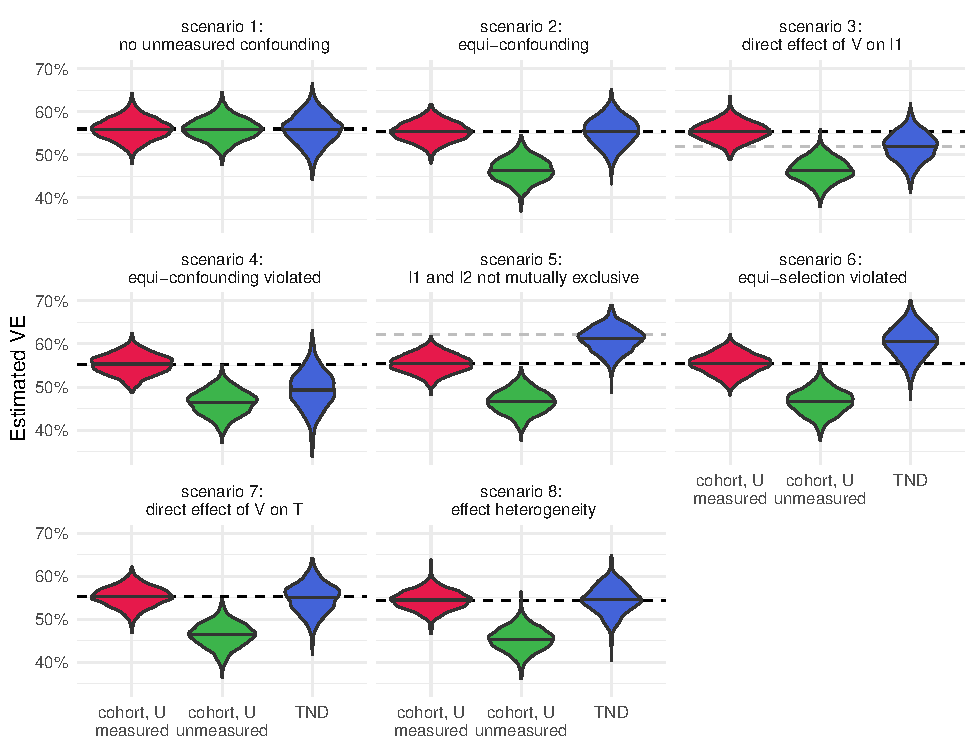
\includegraphics{sims.pdf}
    \caption{Bias of the proposed TND estimator compared to (i) a typical cohort study where $U$ is unmeasured and (ii) an idealized cohort in which $U$ is measured across 9 scenarios representing different true generation processes, based on 1000 Monte Carlo replications. Black dashed line is the true VE. In scenario 3, grey dashed line is the ratio of VEs for test-positive versus test-negative illness. In scenario 5, grey dashed line is one minus the causal odds ratio.}
    \label{fig:sims}
\end{figure}

\clearpage

\begin{appendix}

    \renewcommand{\thefigure}{A\arabic{figure}}
    \setcounter{figure}{0}
    
    \renewcommand{\thetable}{A\arabic{table}}
    \setcounter{table}{0}
    
    \renewcommand{\theequation}{A\arabic{equation}}
    \setcounter{equation}{0}

    \singlespacing
%    \appendixwithtoc
    \newpage

    \section{Proofs of main identifiability results}
    For convenience, we restate the core identifiability assumptions from the main text. 
    \vspace{1em}
    
    \noindent Assumptions:
    \begin{itemize}
        \item[(A1)] Consistency of potential outcomes. For all individuals $i$ and for $v \in \{0, 1\}$, we have $I_i^v = I_i$ and $T_i^v = T_i$ when $V_i = v$.
        \item[(A2)] No effect of vaccination on test-negative symptomatic illness ($I = 1$) among the vaccinated. That is, $\Pr(I^0 = 1 | V = 1, X) = \Pr(I^1 = 1 | V = 1, X).$
        \item[(A3)] Odds ratio equi-confounding. Degree of unmeasured confounding bias on the odds ratio scale is the same for test-positive and test-negative illnesses, i.e. 
        $$\beta_2(X) = \beta_1(X), $$
        $$ \text{where } \beta_i(X) = \log \frac{\Pr(I^0 = i, T^0 = 1 | V = 1, X)\Pr(I^0 = 0, T^0 = 1 | V = 0, X)}{\Pr(I^0 = 0, T^0 = 1 | V = 1, X)\Pr(I^0 = i, T^0 = 1| V = 0, X)}.$$
        \item[(A4)] Overlap of vaccination among test-positives and test-negatives. Define $\mathcal{S}_i(v)$ as the support of the law of $(I^v = i, T^v = 1, V = v, X)$, then for $v$ in $\{0,1\}$, then it must be that $\mathcal{S}_2(1) \subseteq \mathcal{S}_2(0)$ and $\mathcal{S}_2(v) \subseteq \mathcal{S}_1(v).$
        \item[(A5)] No direct effect of vaccination on test-seeking behavior among the vaccinated. That is, for $i$ in $\{1,2\}$, $\Pr[T^1 = 1 | I^1 = i, V = 1, X] = \Pr[T^0 = 1 | I^0 = i, V = 1, X].$
        % \item[(A5)] Equivalent effects of vaccination on test-seeking behavior for test-positive and test-negative illnesses. That is, for $v \in \{0, 1\}$, $\Pr(T^v = 1 | I^v = 2, V = 1, X) = \Pr(T^v = 1 | I^v = 1, V = 1, X)$ and $\Pr(T^v = 1 | I^v = 2, V = 0, X) = \Pr(T^v = 1 | I^v = 1, V = 0, X)$.
    \end{itemize}

    In Proposition \ref{prop1}, we establish that, under consistency alone, the causal risk ratio among the vaccinated, $\Psi_{RRV}$, is equivalent to two expressions involving the (unobserved) treatment-free potential outcome $I^0 = 2$, one based on the outcome itself and one based on the so-called generalized propensity score. In Theorem \ref{theorem1}, we show that, if we add assumptions A2-A4, we can use the observed incidence of the test-negative illness $I = 1$ as a proxy for expressions involved the treatment-free potential outcome, $I^0 = 2$, and therefore identify $\Psi_{RRV}$ if we had access to all symptomatic infections in the underlying cohort. Then in Corollary \ref{corollary1} we show that adding assumption A5 allows us to identify $\Psi_{RRV}$ in the underlying cohort if we only observe infections among those who seek tests. Finally, in Corollary \ref{corollary2} we show $\Psi_{RRV}$ is still identifiable under the sampling design of the TND, due to the invariance of the odds ratio. 
    
    \newpage
    \begin{proposition}\label{prop1}
    Under assumption A1, the causal risk ratio among the vaccinated, 
    \begin{equation*}
        \Psi \equiv \dfrac{\Pr(I^1=2|V=1)}{\Pr(I^0=2|V=1)},
    \end{equation*}
    is equivalent to 
    \begin{equation}
        \Psi^0_{om} \equiv \dfrac{\Pr(I = 2 | V = 1)}{E\left[\Pr(I = 2 | V = 0, X) \exp\{\alpha^0_2(X)\}\Big| V = 1 \right]}
    \end{equation}
    and 
    \begin{equation}
        \Psi^0_{ipw} \equiv \dfrac{E\{V \mathbbm 1(I = 2)\}}{E\left\{ (1 - V) \mathbbm 1(I = 2) \dfrac{\pi^0_2(X)}{1 - \pi^0_2(X)}\right\}}
    \end{equation}
    where 
    \begin{equation*}
        \pi^0_i(X) = \Pr(V = 1 | I^0 = i, X)
    \end{equation*}
    is the generalized propensity score and 
    \begin{equation*}
        \beta^0_i(X) = \log \dfrac{\Pr(I^0 = i | V = 1, X)\Pr(I^0 = 0 | V = 0, X)}{\Pr(I^0 = 0 | V = 1, X)\Pr(I^0 = i | V = 0, X)}
    \end{equation*}
    is the odds ratio comparing the treatment-free potential outcome in the vaccinated and unvaccinated groups with 
    \begin{equation*}
        \eta^0(X) = \log \dfrac{\Pr(I^0 = 0 | V = 0, X)}{\Pr(I^0 = 0 | V = 1, X)}
    \end{equation*}
    and 
    \begin{equation*}
        \alpha^0_i(X) = \log \dfrac{\Pr(I^0 = i | V = 1, X)}{\Pr(I^0 = i | V = 0, X)}
    \end{equation*}
    such that
    \begin{equation*}
        \beta^0_i(X) = \eta^0(X) + \alpha^0_i(X).
    \end{equation*}
    \end{proposition}
    
    \begin{proof}
    For the first expression, we have 
    \begin{align*}
        \Psi &= \dfrac{\Pr(I^1=2|V=1)}{\Pr(I^0=2|V=1)} \\
        &= \dfrac{\Pr(I^1=2|V=1)}{E[E\{\mathbbm 1 (I^0 = 2) | V = 1, X\} | V = 1]} \\
        &= \dfrac{\Pr(I^1=2|V=1)}{E\left\{\int \mathbbm 1 (I^0 = 2) \cdot f(I^0 = i | V = 1, X) di \mid  V = 1\right\}} \\
        &= \dfrac{\Pr(I^1=2|V=1)}{E\left\{\int \mathbbm 1 (I^0 = 2) \cdot f(I^0 = i | V = 0, X) \dfrac{f(I^0 = i | V = 1, X)}{f(I^0 = i | V = 0, X)}di \mid  V = 1\right\}} \\
        &= \dfrac{\Pr(I^1=2|V=1)}{E\left\{ \Pr(I^0 = 2 | V = 0, X) \dfrac{\Pr(I^0 = 2 | V = 1, X)}{\Pr(I^0 = 2 | V = 0, X)} \mid  V = 1\right\}} \\
        &= \dfrac{\Pr(I=2|V=1)}{E\left[ \Pr(I = 2 | V = 0, X) \exp\{\alpha^0_2(X)\} \mid  V = 1\right]}.
    \end{align*}
    The first line restates the definition. The second uses the law of iterated expectation. The third applies the definition of conditional expectation. The fourth multiplies the density by one. The fifth evaluates the integral and the sixth applies consistency and the definition of $\alpha_i(X)$
    
    For the second, we have 
    \begin{align*}
        \Psi &= \dfrac{\Pr(I^1=2|V=1)}{\Pr(I^0=2|V=1)} \\
        &= \dfrac{E\left\{\dfrac{V}{\Pr(V = 1)} \mathbbm 1 (I^1 = 2)\right\}}{E\left\{\dfrac{V}{\Pr(V=1)}\mathbbm 1 (I^0 = 2)\right\}} \\
        &= \dfrac{E\{V \mathbbm 1 (I^1 = 2)\}}{E\left\{\mathbbm 1 (I^0 = 2) E(A | I^0 = 2, X)\right\}} \\
        &= \dfrac{E\{V \mathbbm 1 (I^1 = 2)\}}{E\left\{\mathbbm 1 (I^0 = 2) \pi^0_2(X)\right\}} \\
        &= \dfrac{E\{V \mathbbm 1 (I^1 = 2)\}}{E\left\{\mathbbm 1 (I^0 = 2) \dfrac{\pi^0_2(X)}{1-\pi^0_2(X)}E(1-A|I^0 = 2, X)\right\}} \\
        &= \dfrac{E\{V \mathbbm 1 (I = 2)\}}{E\left\{(1 - V)\mathbbm 1 (I = 2) \dfrac{\pi^0_2(X)}{1-\pi^0_2(X)}\right\}}.
    \end{align*}
    The first line restates the definition. The second uses the definition of conditional expectation. The third applies the law of iterated expectation. The fourth applies the definition of the generalized propensity score $\pi_i(X)$. The fifth multiplies by one. The sixth reverses the law of iterated expectations and applies consistency. 
    \end{proof}
    \newpage
    
    \begin{theorem}\label{theorem1}
    Under assumptions A1 - A4, the causal risk ratio among the vaccinated, 
    \begin{equation*}
        \Psi \equiv \dfrac{\Pr(I^1=2|V=1)}{\Pr(I^0=2|V=1)},
    \end{equation*}
    is identified in the population underlying the test-negative design by 
    \begin{equation}
        \Psi_{om} \equiv \dfrac{\Pr(I = 2 | V = 1)}{E\left\{ \exp\{\alpha_1(X)\} \Pr(I = 2 | V = 0, X) \Big| V = 1 \right\}}
    \end{equation}
    and 
    \begin{equation}
        \Psi_{ipw} \equiv \dfrac{E\{V \mathbbm 1 (I = 2)\}}{E\left\{ (1 - V) \mathbbm 1(I = 2) \dfrac{\pi_1(X)}{1 - \pi_1(X)}\right\}}
    \end{equation}
    where $\alpha_i(X) = \log \dfrac{\Pr(I =i | V = 1, X)}{\Pr(I =i | V = 0, X)}$ and $\pi_i(X) = \Pr(V = 1 | I = i, X)$ are both observables. 
    \end{theorem}
    
    \begin{proof}
    For the first expression, note that by Assumption A3 and exclusivity of test-negative and test-positive illnesses
    \begin{align*}
        \dfrac{\Pr(I^0 = 2 | V = 1, X)}{\Pr(I^0 = 2 | V = 0, X)} &= \dfrac{\Pr(I^0 = 1 | V = 1, X)}{\Pr(I^0 = 1 | V = 0, X)} \\
        &= \dfrac{\Pr(I^1 = 1 | V = 1, X)}{\Pr(I^0 = 1 | V = 0, X)} \\
        &= \dfrac{\Pr(I = 1 | V = 1, X)}{\Pr(I = 1 | V = 0, X)} \\
    \end{align*}
    where the first line is by Assumption A3 and exclusivity of test-negative and test-positive illnesses. The second line is by Assumption A2. And the last line applies consistency. This implies
    \begin{equation*}
        \alpha_2^0(X) = \alpha_1(X)
    \end{equation*}
    and, therefore, combining with the derivation of Proposition \ref{prop1}, we have
    \begin{align*}
        \Psi &= \dfrac{\Pr(I = 2 | V = 1)}{E\left\{ \exp\{\alpha^0_2(X)\} \Pr(I = 2 | V = 0, X) \Big| V = 1 \right\}} \\
        &= \dfrac{\Pr(I = 2 | V = 1)}{E\left\{ \exp\{\alpha_1(X)\} \Pr(I = 2 | V = 0, X) \Big| V = 1 \right\}}.
    \end{align*}
    
    For the second expression, note first that, by the invariance of odds ratios, Assumptions A2 and A3 imply
    \begin{equation*}
        \dfrac{\Pr(V = 1 | I^0 = 2, X)}{\Pr(V = 0 | I^0 = 2, X)} = \dfrac{\Pr(V = 1 | I = 1, X)}{\Pr(V = 0 | I = 1, X)}
    \end{equation*}
    and by consequence 
    \begin{equation*}
        \dfrac{\pi^0_2(X)}{1 - \pi^0_2(X)} = \dfrac{\pi_1(X)}{1 - \pi_1(X)}.
    \end{equation*}
    Thus, again, continuing the derivation in Theorem 1, we have 
    \begin{align*}
        \Psi &= \dfrac{E\{V \mathbbm 1 (I = 2)\}}{E\left\{(1 - V)\mathbbm 1 (I = 2) \dfrac{\pi^0_2(X)}{1-\pi^0_2(X)}\right\}} \\
        &= \dfrac{E\{V \mathbbm 1 (I = 2)\}}{E\left\{(1 - V)\mathbbm 1 (I = 2) \dfrac{\pi_1(X)}{1-\pi_1(X)}\right\}}.
    \end{align*}
    \end{proof}
    \newpage
    
    \begin{corollary}\label{corollary1}
    If we add assumption A5, that is that direct effects of vaccination on testing behavior are the same for test-positive and test-negative illnesses, then $\Psi_{om}$ and $\Psi_{ipw}$ are equivalent to
    \begin{equation}
        \Psi^\dagger_{om} \equiv \dfrac{\Pr(I = 2, T = 1 | V = 1)}{E\left\{ \exp\{\alpha^\dagger_1(X)\} \Pr(I = 2, T = 1 | V = 0, X) \Big| V = 1 \right\}}
    \end{equation}
    and 
    \begin{equation}
        \Psi^\dagger_{ipw} \equiv \dfrac{E\{V \mathbbm 1 (I = 2, T = 1)\}}{E\left\{ (1 - V) \mathbbm 1(I = 2, T = 1) \dfrac{\pi^\dagger_1(X)}{1 - \pi^\dagger_1(X)}\right\}}
    \end{equation}
    where $\alpha^\dagger_1(X) = \dfrac{\Pr(I = 1, T = 1 | V = 1, X)}{\Pr(I = 1, T = 1 | V = 0, X)}$ and $\pi^\dagger_1(X) = \Pr(V = 1| I = 1, T = 1, X)$.
    \end{corollary}
    
    \begin{proof}
        Define $\Psi^\dagger$ as 
        \begin{equation*}
            \Psi^\dagger \equiv  \dfrac{\Pr(I^1=2, T^1 = 1|V=1)}{\Pr(I^0=2, T^0 = 1|V=1)},
        \end{equation*}
        and note that
        \begin{align*}
            \Psi^\dagger &= \dfrac{\Pr(I^1=2, T^1 = 1|V=1)}{\Pr(I^0=2, T^0 = 1|V=1)} \\
            &= \dfrac{\Pr(I^1 = 2 | V = 1)\Pr(T^1 = 1 | I^1 = 2, V = 1)}{\Pr(I^0=2|V=1)\Pr(T^0 = 1 | I^0 = 2, V = 1)} \\
            & = \dfrac{\Pr(I^1 = 2 | V = 1)}{\Pr(I^0 = 2 | V = 1)} \\
            &= \Psi.
        \end{align*}
        The first line follows by definition, the second factors the joint probability, and the third applies applies assumption A3. 
    
        As $\Psi^\dagger = \Psi$, it now suffices to show that $\Psi^\dagger_{om}$ and $\Psi^\dagger_{ipw}$ identify $\Psi^\dagger$. Following the same steps as the derivations in Theorems 1 and 2, for the first expression we have 
        \begin{align*}
        \Psi^\dagger &= \dfrac{\Pr(I^1=2, T^1 = 1|V=1)}{\Pr(I^0=2, T^0 = 1|V=1)} \\
        &= \dfrac{\Pr(I^1=2, T^1 = 1|V=1)}{E[E\{\mathbbm 1 (I^0 = 2, T^0 = 1) | V = 1, X\} | V = 1]} \\
        &= \dfrac{\Pr(I^1=2, T^1 = 1|V=1)}{E\left\{\int \mathbbm 1 (I^0= 2, T^0 = 1) \cdot f(I^0 = i, T^0 = 1 | V = 1, X) di \mid  V = 1\right\}} \\
        &= \dfrac{\Pr(I^1=2, T^1 = 1|V=1)}{E\left\{\int \mathbbm 1 (I^0= 2, T^0 = 1) \cdot f(I^0 = i, T^0 = 1 | V = 0, X) \dfrac{f(I^0 = i, T^0 = 1 | V = 1, X)}{f(I^0 = i, T^0 = 1 | V = 0, X)}di \mid  V = 1\right\}} \\
        &= \dfrac{\Pr(I^1=2, T^1 = 1|V=1)}{E\left\{ \Pr(I^0 = 2, T^0 = 1 | V = 0, X) \dfrac{\Pr(I^0 = 2, T^0 = 1 | V = 1, X)}{\Pr(I^0 = 2, T^0 = 1 | V = 0, X)} \mid  V = 1\right\}} \\
        &= \dfrac{\Pr(I^1=2, T^1 = 1|V=1)}{E\left\{ \Pr(I^0 = 2, T^0 = 1 | V = 0, X) \dfrac{\Pr(I^0 = 1, T^0 = 1 | V = 1, X)}{\Pr(I^0 = 1, T^0 = 1 | V = 0, X)} \mid  V = 1\right\}} \\
        &= \dfrac{\Pr(I^1=2, T^1 = 1|V=1)}{E\left\{ \Pr(I^0 = 2, T^0 = 1 | V = 0, X) \dfrac{\Pr(I^1 = 1, T^1 = 1 | V = 1, X)}{\Pr(I^0 = 1, T^0 = 1 | V = 0, X)} \mid  V = 1\right\}} \\
        &= \dfrac{\Pr(I=2, T = 1|V=1)}{E\left\{ \Pr(I = 2, T = 1 | V = 0, X) \dfrac{\Pr(I = 1, T = 1 | V = 1, X)}{\Pr(I = 1, T = 1 | V = 0, X)} \mid  V = 1\right\}} \\
        &= \dfrac{\Pr(I = 2, T = 1 | V = 1)}{E\left\{ \exp\{\alpha^\dagger_1(X)\} \Pr(I = 2, T = 1 | V = 0, X) \Big| V = 1 \right\}}.
        \end{align*}
    
    For the second expression, note first that, by the invariance of odds ratios, Assumptions A2, A3, and A5 imply
    \begin{equation*}
        \dfrac{\Pr(V = 1 | I^0 = 2, T^0 = 1, X)}{\Pr(V = 0 | I^0 = 2,  T^0 = 1, X)} = \dfrac{\Pr(V = 1 | I = 1, T = 1, X)}{\Pr(V = 0 | I = 1,  T = 1, X)}
    \end{equation*}
    and by consequence 
    \begin{equation*}
        \dfrac{\pi^{0\dagger}_2(X)}{1 - \pi^{0\dagger}_2(X)} = \dfrac{\pi^\dagger_1(X)}{1 - \pi^\dagger_1(X)}.
    \end{equation*}
    Thus we have
    \begin{align*}
        \Psi &= \dfrac{\Pr(I^1=2, T^1 = 1|V=1)}{\Pr(I^0=2, T^0 = 1|V=1)} \\
        &= \dfrac{E\{\dfrac{V}{\Pr(V=1)} \mathbbm 1 (I^1 = 2, T^1 = 1)\}}{E\left\{\dfrac{V}{\Pr(V=1)}\mathbbm 1 (I^0 = 2, T^0 = 1)\right\}} \\
        &= \dfrac{E\{V \mathbbm 1 (I^1 = 2, T^1 = 1)\}}{E\left\{\mathbbm 1 (I^0 = 2, T^0 = 1) E(A | I^0 = 2, T^0 = 1, X)\right\}} \\
        &= \dfrac{E\{V \mathbbm 1 (I^1 = 2, T^1 = 1)\}}{E\left\{\mathbbm 1 (I^0 = 2, T^0 = 1) \pi^{0\dagger}_2(X)\right\}} \\
        &= \dfrac{E\{V \mathbbm 1 (I^1 = 2, T^1 = 1)\}}{E\left\{\mathbbm 1 (I^0 = 2, T^0 = 1) \dfrac{\pi^{0\dagger}_2(X)}{1-\pi^{0\dagger}_2(X)}E(1-A|I^0 = 2, T^0 = 1, X)\right\}} \\
        &= \dfrac{E\{V \mathbbm 1 (I = 2, T = 1)\}}{E\left\{(1 - V)\mathbbm 1 (I = 2, T = 1) \dfrac{\pi^{0\dagger}_2(X)}{1-\pi^{0\dagger}_2(X)}\right\}} \\
        &= \dfrac{E\{V \mathbbm 1 (I = 2, T = 1)\}}{E\left\{(1 - V)\mathbbm 1 (I = 2, T = 1) \dfrac{\pi^\dagger_1(X)}{1-\pi^\dagger_1(X)}\right\}}.
    \end{align*}
    \end{proof}
    \newpage 
    \begin{corollary}\label{corollary2}
    Under assumptions A1 - A5 and the biased sampling design of the test-negative study, $\Psi^\dagger_{om}$ and $\Psi^\dagger_{ipw}$, and therefore by previous results $\Psi_{om}$, $\Psi_{ipw}$, and $\Psi$, are identified by
    \begin{equation}
        \Psi_{om}^* = \dfrac{\Pr(I^* = 1 | S = 1, V = 1)}{E\left\{ \exp\{\alpha^*_1(X)\} \Pr(I^* = 1 | S = 1, V = 0, X) \Big| S = 1, V = 1 \right\}}
    \end{equation}
    and 
    \begin{equation}
        \Psi_{ipw}^* = \dfrac{E\{VI^*|S =1\}}{E\left\{ (1 - V) I^* \dfrac{\pi^*(X)}{1 - \pi^*(X)} \bigg| S = 1\right\}}
    \end{equation}
    where $\alpha^*_1(X) = \dfrac{\Pr(I^* = 0 | S = 1, V = 1, X)}{\Pr(I^* = 0| S = 1, V = 0, X)}$ and $\pi^*(X) = \Pr(V = 1| S = 1, I^* = 0, X)$.
    \end{corollary}
    
    \begin{proof}
    For the first expression we have,
        \begin{align*}
        \Psi^\dagger_{om} &= \dfrac{\Pr(I=2, T = 1|V=1)}{E\left\{ \dfrac{\Pr(I = 1, T = 1 | V = 1, X)}{\Pr(I = 1, T = 1 | V = 0, X)}\Pr(I = 2, T = 1 | V = 0, X) \mid  V = 1\right\}} \\
        &= \dfrac{\Pr(I = 2, T = 1 | V = 1)}{\int \dfrac{\Pr(I = 1, T = 1 | V = 1, x)}{\Pr(I = 1, T = 1 | V = 0, x)} \Pr(I = 2, T = 1 | V = 0, x) f(x | V = 1) dx} \\
        &= \dfrac{\Pr(I = 2 | T = 1, V = 1)\Pr(T = 1 | V = 1)}{\int \dfrac{\Pr(I = 1 | T = 1, V = 1, x)}{\Pr(I = 1 | T = 1, V = 0, x)} \Pr(I = 2 | T = 1, V = 0, x) \Pr(T = 1 | V = 1, x) f(x | V = 1) dx} \\
        &= \dfrac{\Pr(I = 2 | T = 1, V = 1)\Pr(T = 1 | V = 1)}{\int \dfrac{\Pr(I = 1 | T = 1, V = 1, x)}{\Pr(I = 1 | T = 1, V = 0, x)} \Pr(I = 2 | T = 1, V = 0, x) \Pr(T = 1 | V = 1) f(x | T =1, V = 1) dx} \\
        &= \dfrac{\Pr(I = 2 | T = 1, V = 1)}{\int \dfrac{\Pr(I = 1 | T = 1, V = 1, x)}{\Pr(I = 1 | T = 1, V = 0, x)} \Pr(I = 2 | T = 1, V = 0, x) f(x | T =1, V = 1) dx} \\
        &= \dfrac{\Pr(I = 2 | T = 1, V = 1)}{E\left\{ \dfrac{\Pr(I = 1 | T = 1, V = 1, X)}{\Pr(I = 1 | T = 1, V = 0, X)} \Pr(I = 2 | T = 1, V = 0, X) \bigg| T = 1, V = 1\right\}} \\
        &= \dfrac{\Pr(I^* = 1 | S = 1, V = 1)}{E\left\{ \dfrac{\Pr(I^* = 0 | S = 1, V = 1, X)}{\Pr(I^* = 0 | S = 1, V = 0, X)} \Pr(I^* = 1 | S = 1, V = 0, X) \bigg| S = 1, V = 1\right\}} \\
        &= \dfrac{\Pr(I^* = 1 | S = 1, V = 1)}{E\left\{ \exp\{\alpha^*_1(X)\} \Pr(I^* = 1 | S = 1, V = 0, X) \Big| S = 1, V = 1 \right\}}.
    \end{align*}
    The first line restates the definition of $\Psi^\dagger_{om}$. The second applies the definition of conditional expectation. The third factors the joint probabilities. The fourth applies Bayes theorem, i.e. 
    \begin{equation*}
        f(x | V = 1) = \dfrac{f(x | T = 1, V = 1)\Pr(T = 1 | V = 1)}{\Pr(T = 1 | V = 1, x)}.
    \end{equation*}
    The fifth cancels the $\Pr(T = 1 |V = 1)$ terms in the numerator and denominator. The sixth applies the definition of conditional expectation. The seventh applies the sampling design $S = \mathbbm 1 (T = 1, I \neq 0)$ and the perfect test $I^* = \mathbbm 1(I = 2)$.
    
    For the second expression we have,
    \begin{align*}
        \Psi^\dagger_{ipw} &= \dfrac{E\{V \mathbbm 1 (I = 2, T = 1)\}}{E\left\{ (1 - V) \mathbbm 1(I = 2, T = 1) \dfrac{\pi^\dagger_1(X)}{1 - \pi^\dagger_1(X)}\right\}} \\
        &= \dfrac{E\{V \mathbbm 1 (I = 2) | T = 1\} \Pr(T = 1)}{E\left\{ (1 - V) \mathbbm 1(I = 2) \dfrac{\pi^\dagger_1(X)}{1 - \pi^\dagger_1(X)} \bigg| T = 1\right\} \Pr(T = 1)} \\
        &= \dfrac{E\{V \mathbbm 1 (I = 2) | T = 1\}}{E\left\{ (1 - V) \mathbbm 1(I = 2) \dfrac{\pi^\dagger_1(X)}{1 - \pi^\dagger_1(X)} \bigg| T = 1\right\}} \\
        &= \dfrac{E\{VI^*|S =1\}}{E\left\{ (1 - V) I^* \dfrac{\pi^*(X)}{1 - \pi^*(X)} \bigg| S = 1\right\}}.
    \end{align*}
    The first line restates the definition of $\Psi^\dagger_{ipw}$. The second applies the law of iterated expectations. The third cancels the $\Pr(T = 1)$ terms in the numerator and denominator. The fourth applies the sampling design $S = \mathbbm 1 (T = 1, I \neq 0)$ and the perfect test $I^* = \mathbbm 1(I = 2)$.
    
    \end{proof}
    \newpage
    \section{Estimation}
    \subsection{Plug-in}
    Corollary \ref{corollary2} suggests two plug-in estimators for the causal risk ratio among the vaccinated.  An estimator based on modeling the outcome
    \begin{equation}
        \widehat{\Psi}_{om}^* = \dfrac{\sum_{i=1}^n V_i I^*_i}{\sum_{i=1}^n V_i \mu_0(X_i)\dfrac{1 - \mu^*_1(X_i)}{1 - \mu^*_0(X_i)}},
    \end{equation}
    and an inverse probability weighting estimator
    \begin{equation}
        \widehat{\Psi}_{ipw}^* = \dfrac{\sum_{i=1}^n V_i I^*_i}{\sum_{i=1}^n (1 - V_i) I^*_i \dfrac{\pi^*(X_i)}{1 - \pi^*(X_i)}},
    \end{equation}
    where 
    \begin{align*}
        \pi^*(X) &= \Pr(V=1\mid S=1, I^*=0, X) \\
        \mu^*_v(X) &= \Pr(I^*=1\mid S=1, V=v, X).
    \end{align*}

\subsection{Doubly robust}
We consider a 
\begin{equation}\label{eqn:dr_estimator}
\widehat{\Psi}_{dr}^* = \dfrac{\sum_{i=1}^n V_i I^*_i}{\sum_{i=1}^n (1 - V_i)\dfrac{\pi^*_1(X_i)}{1 - \pi^*_1(X_i)} \{I_i - \mu^*_0(X_i) \} + V_i \mu^*_0(X_i)\dfrac{1 - \mu^*_1(X_i)}{1 - \mu^*_0(X_i)}}
\end{equation}

To prove the doubly-robustness of $\widehat{\Psi}^*_{dr}$, it suffices to show that 
\begin{align*}
    E\bigg[ (1 - V)\dfrac{\pi^*_1(X)}{1 - \pi^*_1(X)} \{I - \mu^*_0(X) \} + V \mu^*_0(X)\dfrac{1 - \mu^*_1(X)}{1 - \mu^*_0(X)}\mid S=1\bigg] = \Pi
\end{align*}
if (1) $\dot\mu^*_v(\cdot)=\mu^*_v(\cdot)$ a.s. for $v=0,1$, or (2) $\dot \pi^*(\cdot)=\pi^*(\cdot)$ and $\dot\mu_0(\cdot)=\mu_0(\cdot)$  a.s.

    \begin{enumerate}
        \item If $\dot\mu_v(\cdot)=\mu_v(\cdot)$ a.s. for $v=0,1$, then
        \begin{align*}
            &E\bigg[ (1-V)\{I^* -  \mu_0(X)\}\dfrac{\dot\pi(X)\{1 - \mu_1(X)\}}{\{1 - \dot\pi(X)\}\{1 - \mu_0(X)\}^2} + V\{1-I^*\}\dfrac{\mu_0(X)}{1-\mu_0(X)}\mid S=1\bigg]\\
            =& E\bigg[ \{I^* -  \mu_0(X)\}\dfrac{\dot\pi(X)\{1 - \mu_1(X)\}}{\{1 - \dot\pi(X)\}\{1 - \mu_0(X)\}^2} \mid V=0, S=1\bigg]Pr(V=0\mid  S=1) + \\
            &\qquad E\bigg[E\{V(1-I^*)\mid X\}\dfrac{\mu_0(X)}{1-\mu_0(X)}\mid  S=1\bigg]\\
            =& E\bigg[E \{I^* -  \mu_0(X)\mid V=0, S=1, X\}\dfrac{\dot\pi(X)\{1 - \mu_1(X)\}}{\{1 - \dot\pi(X)\}\{1 - \mu_0(X)\}^2} \mid V=0, S=1\bigg]Pr(V=0\mid  S=1) + \\
            &\qquad E\bigg[\pi(X)\{1-\mu_1(X)\}\dfrac{\mu_0(X)}{1-\mu_0(X)}\mid  S=1\bigg]\\
            &= 0 + \Pi = \Pi
        \end{align*}
    \item If $\dot\pi(\cdot)=\pi(\cdot)$ and $\dot\mu_0(\cdot)=\mu_0(\cdot)$ a.s., then 
\begin{align*}
    &E\bigg[ (1-V)\{I^* -  \mu_0(X)\}\dfrac{\pi(X)\{1 - \dot\mu_1(X)\}}{\{1 - \pi(X)\}\{1 - \mu_0(X)\}^2} + V\{1-I^*\}\dfrac{\mu_0(X)}{1-\mu_0(X)}\mid S=1\bigg]\\
    =& E\bigg[ \{1 - \pi(X)\}\{\mu_0(X) -  \mu_0(X)\}\dfrac{\pi(X)\{1 - \dot\mu_1(X)\}}{\{1 - \pi(X)\}\{1 - \mu_0(X)\}^2} + \pi(X)\{1-\mu_1(X)\}\dfrac{\mu_0(X)}{1-\mu_0(X)}\mid S=1\bigg]\\
    &= \Pi
\end{align*}


    \end{enumerate}
    \subsection{Efficient influence function}
    Let $\Psi(P)$ be the target parameter under true law of the observed data $P$. From the identifiability results in Section 1, we have that 
% $$\Psi(P) = \dfrac{E(I^*\mid S=1, V=1)}{E\left\{\dfrac{\Pr(I^*=1\mid S=1, V=0, X)\Pr(V=1\mid S=1, I^*=0, X)}{\Pr(V=0\mid S=1, I^*=0, X)}\mid S=1, V=1\right\}}.$$ 
$$\Psi(P) = E\left\{\dfrac{\Pr(I^*=1\mid S=1, V=0, X)\Pr(I^*=0\mid S=1, V=1, X)}{\Pr(I^*=0\mid S=1, V=0, X)}\mid S=1, V=1\right\}.$$ 
For convenience, let
\begin{align*}
    \pi(X) &= \Pr(V=1\mid S=1, I^*=0, X) \\
    \mu^*_v(X) &= \Pr(I^*=1\mid S=1, V=v, X).
\end{align*}
Define $P_t$ as a parametric submodel indexed by $t \in [0,1]$ such that
$$P_t = t \widetilde{P} + (1 - t)P$$
where $\widetilde{P}$ is smoothed parametric estimate of $P$ and note that $P_0 = P$. To find the influence function we will use the fact that if we perturb the target in direction of a point mass $\widetilde{o} = (\widetilde{i}^*, \widetilde{s}, \widetilde{v}, \widetilde{x})$ of $\widetilde{P}$
$$ \chi(P, \widetilde{o}) = \frac{d}{dt} \Psi(P_t)\bigg\vert_{t=0}$$
where the right-hand side is the so-called the G\^{a}teaux derivative. Note that 
\begin{align*}
    \Psi(P_t) &= \int \dfrac{\int i^* f_t(i^* | s=1,v=0,x)di^* \int (1-i^*) f_t(i^* | s=1, v=1, x)di^*}{\int(1 - i^*) f_t(i^* | s=1, v=0, x)di^*}f_t(x|s=1,v=1)dx \\
    &= \int \dfrac{1}{f_{S,V}(1, 1)} \dfrac{\int i^* f_t(i^*, s=1,v=0,x)di^* \int (1 - i^*)  f_t(i^*, s=1, v=1, x)dv}{\int(1 - i^*)  f_t(i^*, s=1, v=0, x)dv}dx 
\end{align*}
\begin{align*}
    \Psi(P_t) &= \int (1 - v)i^*\dfrac{\int v f_t(v | s=1, i^*=0, x)dv}{\int (1-v) f_t(v | s=1, i^*=0, x)dv} f(i^*, s=1, v, x) di^* dv dx \\
    &= \int (1 - v)i^*\dfrac{\int v f_t(v, s=1, i^*=0, x)dv}{\int (1-v) f_t(v, s=1, i^*=0, x)dv} f(i^*, s=1, v, x) di^* dv dx
\end{align*}

Then the pathwise derivative of $\Psi_t$ wrt $t$ is
\begin{align*}
   &\frac{d}{dt} \Psi(P_t)\bigg\vert_{t=0} \\
   &= \int \dfrac{1}{f_{S,V}(1, 1)} \frac{d}{dt} \left\{\dfrac{\int i^* f_t(i^*, s=1,v=0,x)di^* \int (1 - i^*)  f_t(i^*, s=1, v=1, x)dv}{\int(1 - i^*)  f_t(i^*, s=1, v=0, x)dv} \right\} \bigg\vert_{t=0}dx \\
   &= \int \dfrac{1}{f_{S,V}(1, 1)}\bigg\{ \dfrac{1 - \mu^*_1(x)}{1-\mu^*_0(x)} \dfrac{f(x, s=1, v=1)}{f(x, s=1, v=0)}\int i^* \frac{d}{dt} f_t(i^*, s=1,v=0,x) \bigg\vert_{t=0} di^* \\
   &\qquad + \dfrac{\mu^*_0(x)}{1 - \mu^*_0(x)} \int (1-i^*) \frac{d}{dt}f_t(i^*, s=1, v=1, x) \bigg\vert_{t=0} di^* \\ 
   &\qquad - \dfrac{\mu^*_0(x)\{1 - \mu^*_1(x)\}}{\{1 - \mu^*_0(x)\}^2} \dfrac{f(x, s=1, v=1)}{f(x, s=1, v =0)} \int (1-i^*) \frac{d}{dt}f_t(i^*, s=1, v=0, x) \bigg\vert_{t=0} dv \\
   % &\qquad + \dfrac{\mu^*_0(x)\pi(x)}{1-\pi(x)} \frac{d}{dt} f_t(x, s=1, v=1) \bigg\vert_{t=0} \\
   % &\qquad - \dfrac{\mu^*_0(x)\pi(x)}{1-\pi(x)} \dfrac{f(x, s=1, v=1)}{f(x, s=1, v=0)} \frac{d}{dt} f_t(x, s=1, v=0) \bigg\vert_{t=0} \bigg\}dx \\
   &= \int \dfrac{1}{f_{S,V}(1, 1)}\bigg\{  \dfrac{1 - \mu^*_1(x)}{1-\mu^*_0(x)} \dfrac{f(x, s=1, v=1)}{f(x, s=1, v=0)}\int i^* \{ \mathbbm 1_{\widetilde i^*, \widetilde s, \widetilde v, \widetilde x}(i^*, 1, 0, x) - f(i^*, s=1,v=0,x) \} di^* \\
   &\qquad + \dfrac{\mu^*_0(x)}{1-\mu^*_0(x)} \int (1 - i^*) \{\mathbbm 1_{\widetilde i^*, \widetilde s, \widetilde v, \widetilde x}(i^*, 1, 1, x) - f(i^*, s=1, v=1, x) \} di^* \\ 
   &\qquad -\dfrac{\mu^*_0(x)\{1 - \mu^*_1(x)\}}{\{1 - \mu^*_0(x)\}^2} \dfrac{f(x, s=1, v=1)}{f(x, s=1, v =0)} \int (1 - i^*) \{\mathbbm 1_{\widetilde i^*, \widetilde s, \widetilde v, \widetilde x}(i^*, 1, 0, x) - f(i^*, s=1, v=0, x) \} di^*  \\
   % & \qquad + \dfrac{\mu^*_0(x)\pi(x)}{1-\pi(x)} \left\{\mathbbm 1_{\widetilde s, \widetilde v, \widetilde x}(1,1,x) - f_t(x, s=1, v=1) \right\} \\
   % & \qquad - \dfrac{\mu^*_0(x)\pi(x)}{1-\pi(x)} \dfrac{f(x, s=1, v=1)}{f(x, s=1, v=0)} \left\{\mathbbm 1_{\widetilde s, \widetilde v, \widetilde x}(1,0,x) - f_t(x, s=1, v=0) \right\}  \bigg\}dx\\
    %&= \int \dfrac{1}{f_{S,V}(1, 1)}\bigg\{ \dfrac{\pi(\widetilde x)}{1-\pi(\widetilde x)} \widetilde i^* \widetilde s(1 - \widetilde v) - \Psi(P) + \dfrac{\mu^*_0(\widetilde x)}{1-\pi(\widetilde x)}(1-\widetilde i^*) \widetilde s \widetilde v  - \Psi(P) - \dfrac{\mu^*_0(x)\pi(x)}{\{1 - \pi(x)\}^2} (1-\widetilde i^*) \widetilde s (1-\widetilde v) - \Psi(P) +  \bigg\}dx \\ 
   &= \int \dfrac{1}{f_{S,V}(1, 1)} \dfrac{\mu^*_0(x)\{1 - \mu^*_1(x)\}}{1 - \mu^*_0(x)}f(x, s=1, v=1) \bigg\{\dfrac{\widetilde{i}^*\widetilde{s}(1-\widetilde{v})\mathbbm 1_{\widetilde{x}}(x)}{\mu^*_0(x)} + \dfrac{(1-\widetilde{i}^*)\widetilde{s}\widetilde{v}\mathbbm 1_{\widetilde{x}}(x)}{1 - \mu^*_1(x)} \\
   &\qquad - \dfrac{(1-\widetilde{i}^*)\widetilde{s}(1-\widetilde{v})\mathbbm 1_{\widetilde{x}}(x)}{\{1 - \mu^*_0(x)\}}\bigg\} dx - \Psi(P) \\
   &=\dfrac{\widetilde s}{f_{S,V}(1, 1)}  \bigg\{(1 - \widetilde v)\widetilde i^*\dfrac{1 - \mu^*_1(\widetilde x)}{1 - \mu^*_0(\widetilde x)} + \widetilde v (1 - \widetilde i^*) \dfrac{\mu^*_0(\widetilde x)}{1 - \mu^*_0(\widetilde x)} -  (1 - \widetilde v) (1 - \widetilde i^*)\dfrac{\mu^*_0(\widetilde x)\{1 - \mu^*_1(\widetilde x)\}}{\{1 - \mu^*_0(\widetilde x)\}^2}  \bigg\}  - \Psi(P) \\
   &=\dfrac{\widetilde s}{f_{S,V}(1, 1)}  \bigg\{(1 - \widetilde v)\widetilde i^*\dfrac{1 - \mu^*_1(\widetilde x)}{1 - \mu^*_0(\widetilde x)} + \widetilde v \left\{\dfrac{\mu^*_0(\widetilde x)}{1 - \mu^*_0(\widetilde x)} - \widetilde i^* \dfrac{\mu^*_0(\widetilde x)}{1 - \mu^*_0(\widetilde x)}\right\} \\
   &\qquad -  (1 - \widetilde v) \left[\dfrac{\mu^*_0(\widetilde x)\{1 - \mu^*_1(\widetilde x)\}}{\{1 - \mu^*_0(\widetilde x)\}^2} - \widetilde i^*\dfrac{\mu^*_0(\widetilde x)\{1 - \mu^*_1(\widetilde x)\}}{\{1 - \mu^*_0(\widetilde x)\}^2}\right]  \bigg\}  - \Psi(P) \\
   &=\dfrac{\widetilde s}{f_{S,V}(1, 1)}  \bigg\{(1 - \widetilde v) \left[\widetilde i^* - \dfrac{\mu^*_0(\widetilde x)}{1 - \mu^*_0(\widetilde x)}  + \widetilde i^*\dfrac{\mu^*_0(\widetilde x)}{1 - \mu^*_0(\widetilde x)}\right]\dfrac{1 - \mu^*_1(\widetilde x)}{1 - \mu^*_0(\widetilde x)}\\
   &\qquad   + \widetilde v \left[\dfrac{\mu^*_0(\widetilde x)}{1 - \mu^*_0(\widetilde x)} - \widetilde i^* \dfrac{\mu^*_0(\widetilde x)}{1 - \mu^*_0(\widetilde x)}\right] \bigg\}  - \Psi(P) \\
   &=\dfrac{\widetilde s}{f_{S,V}(1, 1)}  \bigg\{(1 - \widetilde v) \left[ \dfrac{\widetilde i^* - \widetilde i^* \mu^*_0(\widetilde x) - \mu^*_0(\widetilde x) + \widetilde i^* \mu^*_0(\widetilde x)}{1 - \mu^*_0(\widetilde x)}\right]\dfrac{1 - \mu^*_1(\widetilde x)}{1 - \mu^*_0(\widetilde x)} \\
   &\qquad + \widetilde v \left[\dfrac{\mu^*_0(\widetilde x)}{1 - \mu^*_0(\widetilde x)} - \widetilde i^* \dfrac{\mu^*_0(\widetilde x)}{1 - \mu^*_0(\widetilde x)}\right]   \bigg\}  - \Psi(P) \\
   &=\dfrac{\widetilde s}{f_{S,V}(1, 1)}  \bigg\{(1 - \widetilde v) \{\widetilde i^* - \mu^*_0(\widetilde x)\}\dfrac{1 - \mu^*_1(\widetilde x)}{1 - \mu^*_0(\widetilde x)} + \widetilde v \mu^*_0(\widetilde x) \dfrac{1 - \mu^*_1(\widetilde x)}{1 - \mu^*_0(\widetilde x)}  \bigg\}  - \Psi(P) 
\end{align*}
    \newpage
    
    \section{Example data generation mechanisms satisfying equi-confounding}

    \newpage
    
    \section{Additional results}
    \subsection{Example mechanisms where key assumptions are violated}
    
    \begin{figure}[p]
    \centering
    \begin{subfigure}{0.8\linewidth}
        \centering
        \begin{tikzpicture}[> = stealth, shorten > = 1pt, auto, node distance = 2cm, inner sep = 0pt,minimum size = 0.5pt, semithick]
            \tikzstyle{every state}=[
              draw = none,
              fill = none
            ]
            \node[state] (x) {$X$};
            \node[state] (v) [right of=x] {$V$};
            \node[state] (i) [right of=v] {$I_2$};
            \node[state] (t) [right of=i] {$T$};
            \node[state] (is) [right of=t] {$I^*$};
            \node[state] (i1) [below of=i] {$I_1$};
            \node[state] (u) [below of=x] {$U$};
            \node[state] (v1) [below of=v] {$V_1$};
   
            \path[->] (x) edge node {} (v);
            \path[->] (x) edge [out=45, in=135] node {} (i);
    
            \path[->] (v) edge node {} (i);
            
            \path[->] (i) edge node {} (t);
            \path[->] (i1) edge node {} (t);
            \path[->] (i1) edge node {} (is);

            \path[->] (x) edge [out=45, in=135] node {} (t);
    
            \path[->] (t) edge node {} (is);
            \path[->] (v1) edge node {} (i1);

            \path[->] (i) edge [out=45, in=135] node {} (is);
            \path[->] (i1) edge [dashed] node {} (i);

    
            \path[->] (u) edge node {} (v1);
            \path[->] (u) edge node {} (v);
            % \path[->] (u) edge [line width=2pt] node {} (i);
            % \path[->] (u) edge [line width=2pt] node {} (t);
            % \path[->] (u) edge [line width=2pt] node {} (i1);
            \end{tikzpicture}
        \caption{Correlated vaccination behavior.}
        \end{subfigure}
        \begin{subfigure}{0.8\linewidth}
            \centering
            \begin{tikzpicture}[> = stealth, shorten > = 1pt, auto, node distance = 2.25cm, inner sep = 0pt,minimum size = 0.5pt, semithick]
                \tikzstyle{every state}=[
                  draw = none,
                  fill = none
                ]
                \node[state] (x) {$X$};
                \node[state] (v) [right of=x] {$V$};
                \node[state] (i) [right of=v] {$I_2$};
                \node[state] (t) [right of=i] {$T$};
                \node[state] (is) [right of=t] {$I^*$};
                \node[state] (i1) [below of=i] {$I_1$};
                \node[state] (u) [below of=v] {$U$};
       
                \path[->] (x) edge node {} (v);
                \path[->] (x) edge [out=45, in=135] node {} (i);
        
                \path[->] (v) edge node {} (i);
                
                \path[->] (i) edge node {} (t);
                \path[->] (i1) edge node {} (t);
                \path[->] (i1) edge node {} (is);
    
                \path[->] (x) edge [out=45, in=135] node {} (t);
        
                \path[->] (t) edge node {} (is);
    
                \path[->] (i) edge [out=45, in=135] node {} (is);    
        
                \path[->] (u) edge node {} (v);
                \path[->] (u) edge node {} (i);
                \path[->] (u) edge node {} (t);
                \path[->] (u) edge node {} (i1);
                \end{tikzpicture}
            \caption{$I_1$ and $I_2$ are not mutually exclusive.}
            \end{subfigure}
    % \begin{subfigure}{0.8\linewidth}
    %     \centering
    %     \begin{tikzpicture}[> = stealth, shorten > = 1pt, auto, node distance = 2.25cm, inner sep = 0pt,minimum size = 0.5pt, semithick]
    %         \tikzstyle{every state}=[
    %           draw = none,
    %           fill = none
    %         ]
    %         \node[state] (x) {$X$};
    %         \node[state] (v) [right of=x] {$V$};
    %         \node[state] (i) [right of=v] {$\mathbbm{1}(I = 2)$};
    %         \node[state] (t) [right of=i] {$T$};
    %         \node[state] (is) [right of=t] {$I^*$};
    %         \node[state] (i1) [below of=i] {$\mathbbm{1}(I = 1)$};
    %         \node[state] (u) [below of=v] {$U$};
    
    %         \path[->] (x) edge node {} (v);
    %         \path[->] (x) edge [out=45, in=135] node {} (i);
    
    %         \path[->] (v) edge node {} (i);
            
    %         \path[->] (i) edge node {} (t);
    %         \path[->] (i1) edge node {} (t);
    %         \path[->] (x) edge [out=45, in=135] node {} (t);
    
    %         \path[->] (t) edge node {} (is);
    
    %         \path[->] (i) edge [out=45, in=135] node {} (is);
    
    
    %         \path[->] (i1) edge node {} (i);
    
    
    %         \path[->] (u) edge node {} (x);
    %         \path[->] (u) edge node {} (v);
    %         \path[->] (u) edge node {} (i);
    %         \path[->] (u) edge node {} (t);
    %         \path[->] (u) edge node {} (i1);
            
    %         \end{tikzpicture}
    %     \caption{Splitting $I$ node to show how $I=1$ is a negative outcome control. Solid line is deterministic relationship as $I = 1$ and $I = 2$ are mutually exclusive.}
    %     \end{subfigure}
    %     \begin{subfigure}{0.8\linewidth}
    %         \centering
    %         \begin{tikzpicture}[> = stealth, shorten > = 1pt, auto, node distance = 2.25cm, inner sep = 0pt,minimum size = 0.5pt, semithick]
    %             \tikzstyle{every state}=[
    %               draw = none,
    %               fill = none
    %             ]
    %             \node[state] (x) {$X$};
    %             \node[state] (v) [right of=x] {$V$};
    %             \node[state] (i) [right of=v] {$I$};
    %             \node[state] (z) [right of=i] {$Z$};

    %             \node[state] (t) [right of=z] {$T$};
    %             \node[state] (is) [right of=t] {$I^*$};
    %             \node[state] (u) [below of=v] {$U$};
        
    %             \path[->] (x) edge node {} (v);
    %             \path[->] (x) edge [out=45, in=135] node {} (i);
    %             \path[->] (x) edge [out=45, in=135] node {} (t);
                
    %             \path[->] (v) edge node {} (i);
                
    %             \path[->] (i) edge node {} (z);
    %             \path[->] (i) edge [out=45, in=135] node {} (is);
        
    %             \path[->] (t) edge node {} (is);
        
    %             \path[->] (u) edge node {} (x);
    %             \path[->] (u) edge node {} (v);
    %             \path[->] (u) edge node {} (i);
    %             \path[->] (u) edge node {} (t);
                
    %             \end{tikzpicture}
    %         \caption{Causal directed-acyclic graph for the test-negative design}
    %     \end{subfigure}
    \caption{A}\label{fig:dags}
\end{figure}
\clearpage
\subsection{What if test-positive and test-negative infections are not mutually exclusive?}
Define $I_1$ as an indicator of a symptomatic test-negative infection and $I_2$ as an indicator of a symptomatic test-positive infection, where now we allow for the possibility that $\Pr[I_1 = 1, I_2 = 1] > 0$, but still assume that the symptom screen is effective such that, for any individual $i$, $\mathbbm 1(I_{i,1} + I_{i,2}) = 1$ when $S_i = 1$. We use the following modified assumption set 
\begin{itemize}
    \item[(A1$^\ddagger$)] Consistency of potential outcomes. For all individuals $i$ and for $v \in \{0, 1\}$, we have $I_{2i}^v = I_{2i}$, $I_{1i}^v = I_{1i}$, and $T_i^v = T_i$ when $V_i = v$.
    \item[(A2$^\ddagger$)] No effect of vaccination on test-negative symptomatic illness  among the vaccinated. That is, $\Pr(I_1^0 = 1 | V = 1, X) = \Pr(I_1^1 = 1 | V = 1, X).$
    \item[(A3$^\ddagger$)] Odds ratio equi-confounding. Degree of unmeasured confounding bias on the odds ratio scale is the same for test-positive and test-negative illnesses, i.e. 
        $$\beta_2(X) = \beta_1(X), $$
        $$ \text{where } \beta_i(X) = \log \frac{\Pr(I^0_i = 1, T^0 = 1 | V = 1, X)\Pr(I^0_i = 0, T^0 = 1 | V = 0, X)}{\Pr(I^0_i = 0, T^0 = 1 | V = 1, X)\Pr(I^0_i = 1, T^0 = 1| V = 0, X)}.$$
    \item[(A4$^\ddagger$)] Overlap of vaccination among test-positives and test-negatives. Define $\mathcal{S}_i(v)$ as the support of the law of $(I^v_i, T^v = 1, V = v, X)$, then for $v$ in $\{0,1\}$, then it must be that $\mathcal{S}_2(1) \subseteq \mathcal{S}_2(0)$ and $\mathcal{S}_2(v) \subseteq \mathcal{S}_1(v).$
    \item[(A5$^\ddagger$)] No direct effect of vaccination on test-seeking behavior among the vaccinated. That is, for $i$ in $\{1,2\}$, $\Pr[T^1 = 1 | I^1_i = 1, V = 1, X] = \Pr[T^0 = 1 | I^0_i = 1, V = 1, X].$
\end{itemize}
Here, we show that, under assumptions A1$^\ddagger$-A5$^\ddagger$, the causal odds ratio among the vaccinated remains identified in the test-negative design.

\begin{theorem}
    If the test-negative and test-positive illnesses are not mutually exclusive, then, under assumptions A1$^\ddagger$-A5$^\ddagger$, the causal odds ratio among the vaccinated, 
    \begin{equation*}
        \Phi_{ORV} \equiv \dfrac{\Pr(I^1_2=1|V=1)\Pr(I^1_2=0|V=1)}{\Pr(I^0_2=0|V=1)\Pr(I^0_2=1|V=1)},
    \end{equation*}
    is identified by $\Psi^*_{om}$ and $\Psi^*_{ipw}$ (as defined in Corollary \ref{corollary2}) in the test-negative design.
    \end{theorem}
    
    \begin{proof}
    \begin{align*}
        \Psi_{om}^* &= \dfrac{\Pr(I^* = 1 | S = 1, V = 1)}{E\left\{ \dfrac{\Pr(I^* = 0 | S = 1, V = 1, X)}{\Pr(I^* = 0 | S = 1, V = 0, X)} \Pr(I^* = 1 | S = 1, V = 0, X) \bigg| S = 1, V = 1\right\}} \\
        &= \dfrac{\Pr(I_2 = 1 | S = 1, V = 1)}{E\left\{ \dfrac{\Pr(I_1 = 1, I_2 = 0  | S = 1, V = 1, X)}{\Pr(I_1 = 1, I_2 = 0 | S = 1, V = 0, X)} \Pr(I_2 = 1 | S = 1, V = 0, X) \bigg| S = 1, V = 1\right\}} 
    \end{align*}
    \begin{align*}
        \Phi_{ORV} &= \dfrac{\Pr(I^1_2=1|V=1)\Pr(I^0_2=0|V=1)}{\Pr(I^1_2=0|V=1)\Pr(I^0_2=1|V=1)} \\
        &=\dfrac{\Pr(I^1_2=1, T^1 = 1|V=1)\Pr(I^0_2=0, T^0 = 1|V=1)}{\Pr(I^1_2=0, T^1 = 1|V=1)\Pr(I^0_2=1, T^0 = 1|V=1)} \\
        &=\dfrac{\dfrac{\Pr(I^1_2=1, T^1 = 1|V=1)}{\Pr(I^1_2=0, T^1 = 1|V=1)}}{E\left\{\dfrac{\Pr(I^0_2=1, T^0 =1|V=1, X)}{\Pr(I^0_2=0, T^0 = 1|V=1, X)}\bigg| V = 1\right\}} \\
        &=\dfrac{\dfrac{\Pr(I^1_2=1, T^1 = 1|V=1)}{\Pr(I^1_2=0, T^1 = 1|V=1)}}{E\left\{\dfrac{\dfrac{\Pr(I^0_1=1, T^0 = 1|V=1, X)}{\Pr(I^0_1=0, T^0 = 1|V=1, X)}}{\dfrac{\Pr(I^0_1=1, T^0 = 1|V=0, X)}{\Pr(I^0_1=0, T^0 = 1|V=0, X)}}\dfrac{\Pr(I^0_2=1, T^0 = 1|V=0, X)}{\Pr(I^0_2=0, T^0 = 1|V=0, X)}\bigg| V = 1\right\}} \\
        &=\dfrac{\dfrac{\Pr(I^1_2=1| T^1 = 1, V=1)}{\Pr(I^1_2=0 | T^1 = 1, V=1)}}{E\left\{\dfrac{\dfrac{\Pr(I^0_1=1 | T^0 = 1, V=1, X)}{\Pr(I^0_1=0 | T^0 = 1, V=1, X)}}{\dfrac{\Pr(I^0_1=1 | T^0 = 1, V=0, X)}{\Pr(I^0_1=0 | T^0 = 1, V=0, X)}}\dfrac{\Pr(I^0_2=1 | T^0 = 1, V=0, X)}{\Pr(I^0_2=0 | T^0 = 1,   V=0, X)}\bigg| V = 1\right\}} \\
        &=\dfrac{\dfrac{\Pr(I^1_2=1|V=1)}{\Pr(I^1_2=0|V=1)}}{E\left\{\dfrac{\Pr(I^1_1=1|V=1, X)\Pr(I^0_1=0|V=0, X)}{\Pr(I^1_1=0|V=1, X)\Pr(I^0_1=1|V=0, X)}\dfrac{\Pr(I^0_2=1|V=0, X)}{\Pr(I^0_2=0|V=0, X)}\bigg| V = 1\right\}} \\
        &=\dfrac{\dfrac{\Pr(I_2=1|V=1)}{\Pr(I_2=0|V=1)}}{E\left\{\dfrac{\Pr(I_1=1|V=1, X)\Pr(I_1=0|V=0, X)}{\Pr(I_1=0|V=1, X)\Pr(I_1=1|V=0, X)}\dfrac{\Pr(I_2=1|V=0, X)}{\Pr(I_2=0|V=0, X)}\bigg| V = 1\right\}}
    \end{align*}
    For the first expression, note that by Assumption A3 and exclusivity of test-negative and test-positive illnesses
    \begin{align*}
        \dfrac{\Pr(I^0 = 2 | V = 1, X)}{\Pr(I^0 = 2 | V = 0, X)} &= \dfrac{\Pr(I^0 = 1 | V = 1, X)}{\Pr(I^0 = 1 | V = 0, X)} \\
        &= \dfrac{\Pr(I^1 = 1 | V = 1, X)}{\Pr(I^0 = 1 | V = 0, X)} \\
        &= \dfrac{\Pr(I = 1 | V = 1, X)}{\Pr(I = 1 | V = 0, X)} \\
    \end{align*}
    where the first line is by Assumption A3 and exclusivity of test-negative and test-positive illnesses. The second line is by Assumption A2. And the last line applies consistency. This implies
    \begin{equation*}
        \alpha_2^0(X) = \alpha_1(X)
    \end{equation*}
    and, therefore, combining with the derivation of Theorem 1, we have
    \begin{align*}
        \Psi &= \dfrac{\Pr(I = 2 | V = 1)}{E\left\{ \exp\{\alpha^0_2(X)\} \Pr(I = 2 | V = 0, X) \Big| V = 1 \right\}} \\
        &= \dfrac{\Pr(I = 2 | V = 1)}{E\left\{ \exp\{\alpha_1(X)\} \Pr(I = 2 | V = 0, X) \Big| V = 1 \right\}}.
    \end{align*}
    
    For the second expression, note first that, by the invariance of odds ratios, Assumptions A2 and A3 imply
    \begin{equation*}
        \dfrac{\Pr(V = 1 | I^0 = 2, X)}{\Pr(V = 0 | I^0 = 2, X)} = \dfrac{\Pr(V = 1 | I = 1, X)}{\Pr(V = 0 | I = 1, X)}
    \end{equation*}
    and by consequence 
    \begin{equation*}
        \dfrac{\pi^0_2(X)}{1 - \pi^0_2(X)} = \dfrac{\pi_1(X)}{1 - \pi_1(X)}.
    \end{equation*}
    Thus, again, continuing the derivation in Theorem 1, we have 
    \begin{align*}
        \Psi &= \dfrac{E\{V \mathbbm 1 (I = 2)\}}{E\left\{(1 - V)\mathbbm 1 (I = 2) \dfrac{\pi^0_2(X)}{1-\pi^0_2(X)}\right\}} \\
        &= \dfrac{E\{V \mathbbm 1 (I = 2)\}}{E\left\{(1 - V)\mathbbm 1 (I = 2) \dfrac{\pi_1(X)}{1-\pi_1(X)}\right\}}.
    \end{align*}
    \end{proof}
    \newpage
    
\begin{equation*}
    \Psi = \dfrac{\Pr(I^1_2 = 1 | V = 1)}{\Pr(I^0_2 = 1| V = 1)}
\end{equation*}
Option 1: If tests for $I=1$ and $I=2$ exist 
\begin{equation*}
    \Psi_{ORV} = \dfrac{\Pr(I^1_2 = 1 | V = 1)\Pr(I^0_2 = 0| V = 1)}{\Pr(I^1_2 = 0| V = 1)\Pr(I^0_2 = 1| V = 1)}
\end{equation*}
% \begin{align*}
%     \Pr[I^* = 1 | S = 1, X, V] &= \Pr[I_2 = 1 | S = 1, X, V]\\
%     \Pr[I^* = 0 | S = 1, X, V] &= \Pr[I_1 = 1 | S = 1, X, V] - \Pr[I_2 = 1, I_1 = 1 | S = 1, X, V] 
% \end{align*}
% \begin{align*}
%     \Pr[I_2 = 1 | S = 1, X, V] &= \Pr[I^* = 1 | S = 1, X, V] \\
%     \Pr[I_2 = 0 | S = 1, X, V] &= \Pr[I^* = 0 | S = 1, X, V] \\
%     \Pr[I_1 = 1 | S = 1, X, V] &= \Pr[I^* = 0 | S = 1, X, V] - \Pr[I_2 = 1, I_1 = 1 | S = 1, X, V] \\
%     \Pr[I_1 = 0 | S = 1, X, V] &= \Pr[I^* = 1 | S = 1, X, V]  - \Pr[I_2 = 1, I_1 = 1 | S = 1, X, V] 
% \end{align*}
% \begin{align*}
%     \Pr[I_2 = 1 | S = 1, X, V] &= \Pr[I^* = 1 | S = 1, X, V] \\
%     \Pr[I_2 = 0 | S = 1, X, V] &= \Pr[I^* = 0 | S = 1, X, V] \\
%     \Pr[I_1 = 1 | S = 1, X, V] &= \Pr[I_2 = 0 | S = 1, X, V] - \Pr[I_2 = 1, I_1 = 1 | S = 1, X, V] \\
%     \Pr[I_1 = 0 | S = 1, X, V] &= \Pr[I_2      = 1 | S = 1, X, V]  - \Pr[I_2 = 1, I_1 = 1 | S = 1, X, V] 
% \end{align*}
% % \begin{align*}
% %     \Pr[I_1 = 1 | S = 1, X, V] &= \Pr[I^* = 0 | S = 1, X, V] + \Pr[I_2 = 1, I_1 = 1 | S = 1, X, V] \\
% %     \Pr[I_1 = 0 | S = 1, X, V] &= \Pr[I^* = 1 | S = 1, X, V] - \Pr[I_2 = 1, I_1 = 1 | S = 1, X, V] 
% % \end{align*}
% % and 
% % \begin{align*}
% %     \Pr[I_2 = 1 | S = 1, X, V] &= \Pr[I^* = 1 | S = 1, X, V] \\
% %     \Pr[I_2 = 0 | S = 1, X, V] &= \Pr[I^* = 0 | S = 1, X, V] 
% % \end{align*}
% In this case, Assumption (4) is 
% $$OR_2(X) = OR_1(X), $$
% $$ \text{where } OR_i(X) = \frac{\Pr[I^0_i = 1, T^0 = 1 | V = 1, X]\Pr[I^0_i = 0, T^0 = 1 | V = 0, X]}{\Pr[I^0_i = 0, T^0 = 1 | V = 1, X]\Pr[I^0_i = 1, T^0 = 1| V = 0, X]}.$$
% First, we show that, when $I_1$ and $I_2$ are not mutually exclusive the causal risk ratio is not identified. Following from our previous proof, we have that 
% \begin{align*}
%     \psi_{rrv}(X) &= \phi(X) \times \dfrac{\Pr[I^0_2 = 0, T^0 = 1 | V = 1, X]}{\Pr[I_2 = 0, T = 1 | V = 0, X]}\\
%     \Pr[I_2^0 = 2, T^0 = 1 | V = 1, X] &= \dfrac{\Pr[I_1 = 1, T = 1 | V = 1, X]\Pr[I_1 = 0, T = 1 | V = 0, X]}{\Pr[I_1 = 0, T = 1 | V = 1, X] \Pr[I_1 = 1, T = 1 | V = 0, X]}\\
%     & \quad \quad \times  \dfrac{\Pr[I^0_2 = 0, T^0 = 1 | V = 1, X]}{\Pr[I_2 = 0, T = 1 | V = 0, X]} \Pr[I_2 = 1, T = 1 | V = 0, X]
% \end{align*}

% Here we show that, under these conditions, the conditional odds ratio in the TND identifies the conditional causal odds ratio, i.e.
% \begin{equation*}
%      \psi_{orv}(X) &\equiv \dfrac{\Pr[I^1_2 = 1, T^1 = 1 | V = 1, X]\Pr[I^0_2 = 0, T^0 = 1 | V = 1, X]}{\Pr[I^1_2 = 0, T^1 = 1 | V = 1, X]\Pr[I^0_2 = 1, T^0 = 1 | V = 1, X]}. 
% \end{equation*}

% \begin{align*}
%         \psi_{orv}(X) &= \dfrac{\Pr[I^1_2 = 1, T^1 = 1 | V = 1, X]\Pr[I^0_2 = 0, T^0 = 1 | V = 1, X]}{\Pr[I^1_2 = 0, T^1 = 1 | V = 1, X]\Pr[I^0_2 = 1, T^0 = 1 | V = 1, X]} \\
%         &=  \dfrac{\Pr[I_2 = 1, T = 1 | V = 1, X]\Pr[I^0_2 = 0, T^0 = 1 | V = 1, X]}{\Pr[I_2 = 0, T = 1 | V = 1, X]\Pr[I^0_2 = 1, T^0 = 1 | V = 1, X]} \\
%         &=  \dfrac{\Pr[I_2 = 1, T = 1 | V = 1, X]\Pr[I^0_2 = 0, T^0 = 1 | V = 0, X]}{\Pr[I_2 = 0, T = 1 | V = 1, X]\Pr[I^0_2 = 1, T^0 = 1 | V = 0, X]} \\ & \quad \quad \times \dfrac{\Pr[I^0_1 = 0, T^0 = 1 | V = 1, X]\Pr[I^0_1 = 1, T^0 = 1 | V = 0, X]}{\Pr[I^0_1 = 1, T^0 = 1 | V = 1, X]\Pr[I^0_1 = 0, T^0 = 1| V = 0, X]} \\
%         &=  \dfrac{\Pr[I_2 = 1, T = 1 | V = 1, X]\Pr[I_2 = 0, T = 1 | V = 0, X]}{\Pr[I_2 = 0, T = 1 | V = 1, X]\Pr[I_2 = 1, T = 1 | V = 0, X]} \\ & \quad \quad \times \dfrac{\Pr[I_1 = 0, T = 1 | V = 1, X]\Pr[I_1 = 1, T = 1 | V = 0, X]}{\Pr[I_1 = 1, T = 1 | V = 1, X]\Pr[I_1 = 0, T = 1| V = 0, X]} \\
%         &=  \dfrac{\Pr[I_2 = 1 | I \neq 0, T = 1, V = 1, X]\Pr[I_2 =0 |  I \neq 0, T = 1, V = 0, X]}{\Pr[I_2 = 0 |  I \neq 0, T = 1, V = 1, X]\Pr[I_2 = 1 |  I \neq 0, T = 1, V = 0, X]} \\ & \quad \quad \times \dfrac{\Pr[I_1 = 0 |  I \neq 0, T = 1, V = 1, X]\Pr[I_1 = 1 |  I \neq 0, T = 1, V = 0, X]}{\Pr[I_1 = 1 |  I \neq 0, T = 1, V = 1, X]\Pr[I_1 = 0 |  I \neq 0, T = 1, V = 0, X]}\\
%         &=  \dfrac{\Pr[I_2 = 1 | S = 1, V = 1, X]\Pr[I_2 =0 |  S = 1, V = 0, X]}{\Pr[I_2 = 0 |  S = 1, V = 1, X]\Pr[I_2 = 1 | S = 1, V = 0, X]} \\ & \quad \quad \times \dfrac{\Pr[I_1 = 0 |  S = 1, V = 1, X]\Pr[I_1 = 1 |  S = 1, V = 0, X]}{\Pr[I_1 = 1 |  S = 1, V = 1, X]\Pr[I_1 = 0 |  S = 1, V = 0, X]}\\
%         &=  \dfrac{\Pr[I^* = 1 | S = 1, V = 1, X]}{\Pr[I^* = 0|  S = 1, V = 1, X]} \dfrac{\Pr[I^* = 0 |  S = 1, V = 0, X]}{\Pr[I^* = 1 | S = 1, V = 0, X]}\\
% \end{align*}  
    
% Note that in this case, Assumption (4) becomes 
% \begin{itemize}
%      \item[(A4)] Odds ratio equi-confounding. Degree of unmeasured confounding bias on the odds ratio scale is the same for all symptomatic illness regardless if $I_1$ or $I_2$ is cause, i.e. 
%     $$OR_2(X) = OR_1(X), $$
%     $$ \text{where } OR_i(X) = \frac{\Pr[I^0_i = 1, T^0 = 1 | V = 1, X]\Pr[I^0_i = 0, T^0 = 1 | V = 0, X]}{\Pr[I^0_i = 0, T^0 = 1 | V = 1, X]\Pr[I^0_i = 1, T^0 = 1| V = 0, X]}.$$
% \end{itemize}
% Consider the conditional odds ratio for the effect of vaccination among the vaccinated, i.e.
%     \begin{align*}
%         \psi_{orv}(X) &\equiv \dfrac{\Pr[I^1_2 = 1, T^1 = 1 | V = 1, X]\Pr[I^0_2 = 0, T^0 = 1 | V = 1, X]}{\Pr[I^1_2 = 0, T^1 = 1 | V = 1, X]\Pr[I^0_2 = 1, T^0 = 1 | V = 1, X]} \\
%         &=  \dfrac{\Pr[I_2 = 1, T = 1 | V = 1, X]\Pr[I^0_2 = 0, T^0 = 1 | V = 1, X]}{\Pr[I_2 = 0, T = 1 | V = 1, X]\Pr[I^0_2 = 1, T^0 = 1 | V = 1, X]} \\
%         &=  \dfrac{\Pr[I_2 = 1, T = 1 | V = 1, X]\Pr[I^0_2 = 1, T^0 = 1 | V = 0, X]}{\Pr[I_2 = 0, T = 1 | V = 1, X]\Pr[I^0_2 = 0, T^0 = 1 | V = 0, X]} \\ & \quad \quad \times \dfrac{\Pr[I^0_1 = 1, T^0 = 1 | V = 1, X]\Pr[I^0_1 = 0, T^0 = 1 | V = 0, X]}{\Pr[I^0_1 = 0, T^0 = 1 | V = 1, X]\Pr[I^0_1 = 1, T^0 = 1| V = 0, X]} \\
%         &=  \dfrac{\Pr[I_2 = 1, T = 1 | V = 1, X]\Pr[I_2 = 1, T = 1 | V = 0, X]}{\Pr[I_2 = 0, T = 1 | V = 1, X]\Pr[I_2 = 0, T = 1 | V = 0, X]} \\ & \quad \quad \times \dfrac{\Pr[I_1 = 1, T = 1 | V = 1, X]\Pr[I_1 = 0, T = 1 | V = 0, X]}{\Pr[I_1 = 0, T = 1 | V = 1, X]\Pr[I_1 = 1, T = 1| V = 0, X]}
%     \end{align*}        
% Under the consistency assumption (A1) the numerator is equal to $\Pr[I = 2, T = 1 | V = 1, X]$. Focusing on the denominator, under equi-confounding (A3)
% \begin{equation*}
% \Pr[I^0 = 2, T^0 = 1  | V = 1, X] = \frac{\Pr[I^0 = 1, T^0 = 1  | V = 1, X]}{\Pr[I^0 = 1, T^0 = 1  | V = 0, X]}\Pr[I^0 = 2, T^0 = 1 | V = 0, X]
% \end{equation*}
% and then by (A1) and (A2) with (A4) ensuring overlap
%     \begin{equation*}
%      \Pr[I^0 = 2, T^0 = 1  | V = 1, X] = \frac{\Pr[I = 1, T = 1  | V = 1, X]}{\Pr[I = 1, T = 1  | V = 0, X]}\Pr[I = 2, T = 1 | V = 0, X]
%     \end{equation*}
% Plugging back into the expression for $\psi_{rrv}(X)$, we find the following identifying expression 
%     \begin{equation*}
%          \phi(X) \equiv \dfrac{\dfrac{\Pr[I = 2, T = 1 | V = 1, X]}{\Pr[I = 1, T = 1 | V = 1, X]}}{\dfrac{\Pr[I = 2, T = 1 | V = 0, X]}{\Pr[I = 1, T = 1 | V = 0, X]}}
%     \end{equation*}
% which is the ratio of the odds of symptomatic infection with the vaccine pathogen versus symptomatic infection with another pathogen in the vaccinated and unvaccinated. It is also strictly written in terms of the observables. A key insight is that $\frac{\Pr[I = 1, T =1  | V = 0, X]}{\Pr[I = 1, T = 1 | V = 1, X]}$ acts as a proxy for $\frac{\Pr[I^0 = 2, T =1  | V = 0, X]}{\Pr[I^0 = 2, T = 1 | V = 1, X]}$ essentially a ``parallel trend'' for $I=2$ in absence of vaccination.

% Recall that, in a test-negative study, we only observe test results among the symptomatic and tested, i.e. samples $\{(X_i, V_i, S_i = 1, I^*_i) : i = 1, \ldots, n\}$ where $S = \mathbb{I}(I \neq 0, T = 1)$. However, we can show that 
%     \begin{align*}
%          \phi(X) &= \dfrac{\dfrac{\Pr[I^* = 1 | S = 1, V = 1, X]}{\Pr[I^* = 0 | S = 1, V = 1, X]}}{\dfrac{\Pr[I^* = 1 | S = 1, V = 0, X]}{\Pr[I^* = 0 | S = 1, V = 0, X]}}
%     \end{align*}    
% which is the odds ratio comparing odds of testing positive for vaccinated and unvaccinated among the tested only.
\newpage 
\subsection{What if there is a direct effect of vaccination on testing behavior?}
Unlike in a placebo-controlled trial, participants in a test-negative design are generally aware of their vaccination status. It is therefore possible that this knowledge could affect their testing behavior in a number of ways which would violate Assumption A5. For instance, some individuals may be less likely to get tested when vaccinated because they feel more protected or perceive the risk of illness to be lower. Here, we consider identifiability under a weaker assumption A5*:
\begin{itemize}
    \item[(A5*)] Equivalent effects of vaccination on test-seeking behavior for test-positive and test-negative illnesses among the vaccinated. That is, 
    \begin{equation}
    \dfrac{\Pr(T^1 = 1 | I^1 = 1, V = 1, X)}{\Pr(T^0 = 1 | I^0 = 1, V = 1, X)} = \dfrac{\Pr(T^1 = 1 | I^1 = 2, V = 1, X)}{\Pr(T^0 = 1 | I^0 = 2, V = 1, X)}.
\end{equation}
\end{itemize}
This assumption allows for vaccination to affect testing behavior provided it does so similarly for test-positive and test-negative illnesses. Together with assumption A4 it implies
\begin{equation*}
    \dfrac{\Pr(T = 1 | I = 1, V = 1, X)}{\Pr(T = 1 | I = 1, V = 0, X)} = \dfrac{\Pr(T = 1 | I = 2, V = 1, X)}{\Pr(T = 1 | I = 2, V = 0, X)}.
\end{equation*}
It may be plausible given that participants may not know which infection they have prior to receiving a test. Note that, it would still be violated if vaccination reduced severity or altered symptoms of infection, and therefore willingness to seek a test, for $I=2$ but not $I=1$. In Corollary 3, we show that under this assumption we can still identify the causal risk ratio among the vaccinated in the test-negative study. 
\vspace{1em}

% \begin{equation}
%     \dfrac{\Pr(T^1 = 1 | I^1 = 1, V = 1, X)}{\Pr(T^0 = 1 | I^0 = 1, V = 1, X)} = \dfrac{\Pr(T^1 = 1 | I^1 = 2, V = 1, X)}{\Pr(T^0 = 1 | I^0 = 2, V = 1, X)}
% \end{equation}

% \begin{align*}
%     \Pr&(T^1 = 1 | I^1 = 1, V = 1, X) \\
%     &= \dfrac{\Pr(T^1 = 1 | I^1 = 2, V = 1, X)}{\Pr(T^0 = 1 | I^0 = 2, V = 1, X)}\Pr(T^0 = 1 | I^0 = 1, V = 1, X) \\
%     &= \dfrac{\Pr(T^1 = 1 | I^1 = 2, V = 1, X)\Pr(T^0 = 1 | I^0 = 1, V = 0, X)\Pr(T^0 = 1 | I^0 = 1, V = 1, X)}{\Pr(T^0 = 1 | I^0 = 1, V = 1, X)\Pr(T^0 = 1 | I^0 = 2, V = 0, X)} \\
%      &= \dfrac{\Pr(T^1 = 1 | I^1 = 2, V = 1, X)\Pr(T^0 = 1 | I^0 = 1, V = 0, X)}{\Pr(T^0 = 1 | I^0 = 2, V = 0, X)} \\
% \end{align*}

% \begin{align*}
%     \Pr&(T^0 = 1 | I^0 = 1, V = 1, X) \\
%     &= \dfrac{\Pr(T^0 = 1 | I^0 = 2, V = 1, X)}{\Pr(T^1 = 1 | I^1 = 2, V = 1, X)} \Pr(T^1 = 1 | I^1 = 1, V = 1, X)\\
%     &= \dfrac{\Pr(T^0 = 1 | I^0 = 1, V = 1, X)\Pr(T^0 = 1 | I^0 = 2, V = 0, X)\Pr(T^1 = 1 | I^1 = 1, V = 1, X)}{\Pr(T^1 = 1 | I^1 = 2, V = 1, X)\Pr(T^0 = 1 | I^0 = 1, V = 0, X)} \\
%      1 &= \dfrac{\Pr(T^0 = 1 | I^0 = 2, V = 0, X)\Pr(T^1 = 1 | I^1 = 1, V = 1, X)}{\Pr(T^1 = 1 | I^1 = 2, V = 1, X)\Pr(T^0 = 1 | I^0 = 1, V = 0, X)} \\
% \end{align*}
    

\begin{corollary}
    Under assumptions A1-A4 and alternative assumption A5* that direct effects of vaccination on testing behavior are the same for test-positive and test-negative illnesses, $\Psi$ is identified by $\Psi^\dagger_{om}$ and $\Psi^\dagger_{ipw}$ (as defined in Corollary \ref{corollary1}) in the full cohort as well as $\Psi^*_{om}$ and $\Psi^*_{ipw}$ (as defined in Corollary \ref{corollary2}) in the test-negative design.
\end{corollary}
    
    \begin{proof}
        Define $\Psi^\dagger$ as 
        \begin{equation*}
            \Psi^\dagger \equiv  \dfrac{\Pr(I^1=2, T^1 = 1|V=1)}{\Pr(I^0=2, T^0 = 1|V=1)},
        \end{equation*}
        and note that
        \begin{align*}
            \Psi^\dagger &= \dfrac{\Pr(I^1=2|V=1)}{\Pr(I^0=2|V=1)} \\
            &= \dfrac{\Pr(I^1=2|V=1)}{\Pr(I^0=2|V=1)} \dfrac{\Pr(T = 1 | I = 2, V = 1, X)}{\Pr(T = 1 | I = 2, V = 0, X)}\dfrac{\Pr(T = 1 | I = 1, V = 0, X)}{\Pr(T = 1 | I = 1, V = 1, X)}\\
            & = \dfrac{\Pr(I^1 = 2 | V = 1)}{E\left\{\dfrac{\Pr(I^0 = 2, T^0 = 1 | V = 1, X)}{\Pr(T^1 = 1 | I^1 = 2, V = 1, X)}  \bigg| V = 1\right\}} \\
            & = \dfrac{\Pr(I^1 = 2 | V = 1)}{E\left\{\dfrac{\Pr(I^0 = 1, T^0 = 1 | V = 1, X)\Pr(I^0 = 2, T^0 = 1 | V = 0, X)}{\Pr(I^0 = 1, T^0 = 1 | V = 0, X)\Pr(T^1 = 1 | I^1 = 2, V = 1, X)}  \bigg| V = 1\right\}} \\
            & = \dfrac{\Pr(I^1 = 2 | V = 1)}{E\left\{\dfrac{\Pr(I^1 = 1 | V = 1, X)}{\Pr(I^0 = 1 | V = 0, X)}\Pr(I^0 = 2 | V = 0, X)  \bigg| V = 1\right\}} \\
            & = \dfrac{\Pr(I^1 = 2 | V = 1)}{E\left\{\Pr(I^0 = 2 | V = 1, X)  \bigg| V = 1\right\}} \\
            & = \dfrac{\Pr(I^1 = 2 | V = 1)}{\Pr(I^0 = 2 | V = 1)} \\
            &= \Psi.
        \end{align*}
        The first line follows by definition. The second factors the joint probability. The third applies the law of iterated expectations. The fourth applies assumption A3. The fifth applies assumption A5. The sixth reverses assumption A3 and the seventh reverses the law of iterated expectations. 
    
        As $\Psi^\dagger = \Psi$, it now suffices to show that $\Psi^\dagger_{om}$ and $\Psi^\dagger_{ipw}$ identify $\Psi^\dagger$. Following the same steps as the derivations in Theorems 1 and 2, for the first expression we have 
        \begin{align*}
        \Psi^\dagger &= \dfrac{\Pr(I^1=2, T^1 = 1|V=1)}{\Pr(I^0=2, T^0 = 1|V=1)} \\
        &= \dfrac{\Pr(I^1=2, T^1 = 1|V=1)}{E[E\{\mathbbm 1 (I^0 = 2, T^0 = 1) | V = 1, X\} | V = 1]} \\
        &= \dfrac{\Pr(I^1=2, T^1 = 1|V=1)}{E\left\{\int \mathbbm 1 (I^0= 2, T^0 = 1) \cdot f(I^0 = i, T^0 = 1 | V = 1, X) di \mid  V = 1\right\}} \\
        &= \dfrac{\Pr(I^1=2, T^1 = 1|V=1)}{E\left\{\int \mathbbm 1 (I^0= 2, T^0 = 1) \cdot f(I^0 = i, T^0 = 1 | V = 0, X) \dfrac{f(I^0 = i, T^0 = 1 | V = 1, X)}{f(I^0 = i, T^0 = 1 | V = 0, X)}di \mid  V = 1\right\}} \\
        &= \dfrac{\Pr(I^1=2, T^1 = 1|V=1)}{E\left\{ \Pr(I^0 = 2, T^0 = 1 | V = 0, X) \dfrac{\Pr(I^0 = 2, T^0 = 1 | V = 1, X)}{\Pr(I^0 = 2, T^0 = 1 | V = 0, X)} \mid  V = 1\right\}} \\
        &= \dfrac{\Pr(I^1=2, T^1 = 1|V=1)}{E\left\{ \Pr(I^0 = 2, T^0 = 1 | V = 0, X) \dfrac{\Pr(I^0 = 1, T^0 = 1 | V = 1, X)}{\Pr(I^0 = 1, T^0 = 1 | V = 0, X)} \mid  V = 1\right\}} \\
        &= \dfrac{\Pr(I^1=2, T^1 = 1|V=1)}{E\left\{ \Pr(I^0 = 2, T^0 = 1 | V = 0, X) \dfrac{\Pr(I^1 = 1, T^1 = 1 | V = 1, X)}{\Pr(I^0 = 1, T^0 = 1 | V = 0, X)} \mid  V = 1\right\}} \\
        &= \dfrac{\Pr(I=2, T = 1|V=1)}{E\left\{ \Pr(I = 2, T = 1 | V = 0, X) \dfrac{\Pr(I = 1, T = 1 | V = 1, X)}{\Pr(I = 1, T = 1 | V = 0, X)} \mid  V = 1\right\}} \\
        &= \dfrac{\Pr(I = 2, T = 1 | V = 1)}{E\left\{ \exp\{\alpha^\dagger_1(X)\} \Pr(I = 2, T = 1 | V = 0, X) \Big| V = 1 \right\}}.
        \end{align*}
    
    For the second expression, note first that, by the invariance of odds ratios, Assumptions A2, A3, and A5 imply
    \begin{equation*}
        \dfrac{\Pr(V = 1 | I^0 = 2, T^0 = 1, X)}{\Pr(V = 0 | I^0 = 2,  T^0 = 1, X)} = \dfrac{\Pr(V = 1 | I = 1, T = 1, X)}{\Pr(V = 0 | I = 1,  T = 1, X)}
    \end{equation*}
    and by consequence 
    \begin{equation*}
        \dfrac{\pi^{0\dagger}_2(X)}{1 - \pi^{0\dagger}_2(X)} = \dfrac{\pi^\dagger_1(X)}{1 - \pi^\dagger_1(X)}.
    \end{equation*}
    Thus we have
    \begin{align*}
        \Psi &= \dfrac{\Pr(I^1=2, T^1 = 1|V=1)}{\Pr(I^0=2, T^0 = 1|V=1)} \\
        &= \dfrac{E\{\dfrac{V}{\Pr(V=1)} \mathbbm 1 (I^1 = 2, T^1 = 1)\}}{E\left\{\dfrac{V}{\Pr(V=1)}\mathbbm 1 (I^0 = 2, T^0 = 1)\right\}} \\
        &= \dfrac{E\{V \mathbbm 1 (I^1 = 2, T^1 = 1)\}}{E\left\{\mathbbm 1 (I^0 = 2, T^0 = 1) E(A | I^0 = 2, T^0 = 1, X)\right\}} \\
        &= \dfrac{E\{V \mathbbm 1 (I^1 = 2, T^1 = 1)\}}{E\left\{\mathbbm 1 (I^0 = 2, T^0 = 1) \pi^{0\dagger}_2(X)\right\}} \\
        &= \dfrac{E\{V \mathbbm 1 (I^1 = 2, T^1 = 1)\}}{E\left\{\mathbbm 1 (I^0 = 2, T^0 = 1) \dfrac{\pi^{0\dagger}_2(X)}{1-\pi^{0\dagger}_2(X)}E(1-A|I^0 = 2, T^0 = 1, X)\right\}} \\
        &= \dfrac{E\{V \mathbbm 1 (I = 2, T = 1)\}}{E\left\{(1 - V)\mathbbm 1 (I = 2, T = 1) \dfrac{\pi^{0\dagger}_2(X)}{1-\pi^{0\dagger}_2(X)}\right\}} \\
        &= \dfrac{E\{V \mathbbm 1 (I = 2, T = 1)\}}{E\left\{(1 - V)\mathbbm 1 (I = 2, T = 1) \dfrac{\pi^\dagger_1(X)}{1-\pi^\dagger_1(X)}\right\}}.
    \end{align*}
    \end{proof}

\newpage
\subsection{What if symptom screen is imperfect?}
Here we mean what if some non
\newpage
\subsection{What if test is imperfect?}
Recall that 

$$\Pr[I^* = 1 | S = 1, V = 1, X] = \Pr[I = 2 | S = 1, V = 1, X] \Pr[I^* = 1]$$

$I^* = \lambda_{sens} \cdot \mathbb{I}(I = 2) + (1 - \lambda_{spec}) \cdot \mathbb{I}(I \neq 2)$

\subsection{What about immortal time bias?}

\subsection{Relationship to vaccination mechanisms}
% Define the following:
% \begin{description}
%     \item[$\lambda$:] Force of infection 
%     \item[$\pi$:] Probability of symptoms given infection
%     \item[$P$:] Total population 
%     \item[$v$:] Proportion vaccinated
%     \item[$\mu$:] Probability of care-seeking given symptoms
%     \item[$\theta(t):$] Hazard ratio for infection given 
% \end{description}
% The rate of ascertaining test-positive, vaccinated persons is
% $$
% \Lambda_{V I}(t)=\lambda_I \pi_I \mu_V[(1-\varphi) e^{-\lambda_I t} + \varphi \theta e^{-\theta \lambda_I t}] v P .
% $$

% $$
% \Lambda_{U I}(t)=\lambda_I \pi_I \mu_U e^{-\lambda_I t}(1-v) P .
% $$

% Test-negative vaccinated and unvaccinated persons are ascertained at the rates
% $$
% \Lambda_{V N}(t)=\lambda_N \pi_N \mu_V v P
% $$
% and
% $$
% \Lambda_{U N}(t)=\lambda_N \pi_N \mu_U(1-v) P,
% $$
% respectively, assuming vaccination does not affect susceptibility to the test-negative conditions.

% Test-negative studies typically measure the odds ratio of vaccination among the test-positive and test-negative subjects, similar to the exposure odds ratio in case-control studies, using cumulative cases $(C)$. For the test-positive outcome,
% $$
% \begin{gathered}
% C_{V I}(t)=\pi_I \mu_V\left[(1-\varphi)\left(1-e^{-\lambda_I t}\right)+\varphi\left(1-e^{-\theta \lambda_I t}\right)\right] v P \\
% C_{U I}(t)=\pi_I \mu_U\left(1-e^{-\lambda_I t}\right)(1-v) P .
% \end{gathered}
% $$

% Under the assumption that test-negative infections are not immunizing, cumulative cases are proportional to the incidence rate and study duration:
% $$
% \begin{gathered}
% C_{V N}(t)=\lambda_N \pi_N \mu_V v P t \\
% C_{U N}(t)=\lambda_N \pi_N \mu_U(1-v) P t .
% \end{gathered}
% $$

% We consider the case of immunizing test-negative outcomes in Web Appendix 1. Using the vaccine-exposure odds ratio measured from cumulative cases,
% $$
% \begin{aligned}
% 1-O R^C(t) & =1-\frac{C_{V I}(t) C_{U N}(t)}{C_{U I}(t) C_{V N}(t)} \\
% & =1-\frac{(1-\varphi)\left(1-e^{-\lambda_I t}\right)+\varphi\left(1-e^{-\theta \lambda_I t}\right)}{1-e^{-\lambda_I t}} \\
% & =\varphi\left(1-\frac{1-e^{-\theta \lambda_I t}}{1-e^{-\lambda_I t}}\right) .
% \end{aligned}
% $$

% $\varphi$
\end{appendix}



\end{document}